\documentclass[12pt,a4paper]{amsart}
\usepackage{a4}
%%%%%%%%%%%%%
\usepackage[utf8]{inputenc}
\usepackage[T1]{fontenc}
\usepackage{amsmath}
\usepackage{amsfonts,amssymb,amsthm}
\usepackage[color=green!30]{todonotes}
\usepackage{xcolor}
\usepackage{enumitem}
\usepackage[colorlinks,
    linkcolor={red!50!black},
    citecolor={blue!50!black},
    urlcolor={blue!80!black}]{hyperref}
\usepackage[noabbrev,nameinlink,capitalise]{cleveref}
\usepackage[xy]{qsymbols}
\usepackage{tikz-cd}
\usetikzlibrary{arrows}
%\newcommand{\midarrow}{\tikz \draw[-triangle 90] (0,0) -- +(.1,0);}
\usepackage{mathtools}
%\usepackage{nicematrix}
\usepackage{array,arydshln}
\usepackage{bigdelim}
 \usetikzlibrary {arrows.meta} 
 \usepackage{mathrsfs}
 \usepackage{graphicx,scalerel}
 \newcommand\wh[1]{\hstretch{3}{\hat{\hstretch{0.33}{#1\kern+0.12em}}}}

\DeclareMathOperator{\Sym}{Sym}
\DeclareMathOperator{\GL}{GL}
\DeclareMathOperator{\PSL}{PSL}
\DeclareMathOperator{\PGL}{PGL}
\DeclareMathOperator{\PSU}{PSU}
\DeclareMathOperator{\SU}{SU}
\DeclareMathOperator{\SO}{SO}
\DeclareMathOperator{\SL}{SL}
\DeclareMathOperator{\Tr}{Tr}
\DeclareMathOperator{\Hom}{Hom}
\DeclareMathOperator{\tor}{tor}
\newcommand{\RR}{\mathbb R}
\newcommand{\CC}{\mathbb C}
\newcommand{\ZZ}{\mathbb Z}
\newcommand{\QQ}{\mathbb Q}
\newcommand{\HH}{\mathbb H}
\DeclareMathOperator{\Id}{Id}
\newcommand{\bma}{\begin{pmatrix}}
\newcommand{\ema}{\end{pmatrix}}
\newcommand{\bsm}{\left(\begin{smallmatrix}}
\newcommand{\esm}{\end{smallmatrix}\right)}
\newcommand{\dd}{\mathrm{d}}
\DeclareMathOperator{\vN}{vN}
\newcommand{\detFK}{{\det}_{\mathrm{FK}}}
\renewcommand{\Re}{\operatorname{Re}}
\DeclareMathOperator{\Vol}{Vol}
\DeclareMathOperator{\lk}{lk}
\DeclareMathOperator{\im}{im}
\DeclareMathOperator{\tr}{tr}
\newcommand{\bs}[1]{{\boldsymbol{#1}}}
%\newcommand{\norm}[1]{\left||{#1}\right||}
\newcommand{\norm}[1]{\lVert{#1}\rVert}

\newtheorem{theorem}{Theorem}
\newtheorem{conj}{Conjecture}
\newtheorem{corollary}[theorem]{Corollary}
\newtheorem{lemma}[theorem]{Lemma}
\newtheorem{proposition}[theorem]{Proposition}
\newtheorem{question}[theorem]{Question}
\newtheorem{conjecture}[theorem]{Conjecture}
\newtheorem*{thmintro}{Theorem}
\newtheorem*{claim}{Claim}
\newtheorem*{notation}{Notation}

\theoremstyle{definition}
\newtheorem{definition}[theorem]{Definition}
\newtheorem{terminology}{Terminology}
\newtheorem{example}[theorem]{Example}

\newtheorem{remark}[theorem]{Remark}
\newtheorem{construction}[theorem]{Construction}

%Titre & divers
%\subjclass[2000]{Primary: 57M25, Secondary: 57M27}
\keywords{}

\crefname{collitem}{}{}
\creflabelformat{collitem}{#2\cref{prop:collect}~(#1)#3}

\begin{document}
\title[Triangulations and combinatorial zeta functions]{Combinatorial zeta functions counting triangles}
%\date{\today}
\author{Leo Benard}
\address{Mathematisches Institut, Georg--August Universit\"at G\"ottingen $\&$
Institut de Mathématiques de Marseille, Aix--Marseille University}
\email{leo.benard@univ-amu.fr}
\author{Yann Chaubet}
\address{Department of Pure Mathematics and Mathematical Statistics, University of
Cambridge, Cambridge}
\email{y.chaubet@dpmms.cam.ac.uk}
\author{Nguyen Viet Dang}
\address{Sorbonne Université and Université Paris Cité, CNRS, IMJ-PRG, F-75005 Paris, France.\\
Institut Universitaire de France, Paris, France.}
\email{dang@imj-prg.fr }
\author{Thomas Schick}
\address{Mathematisches Institut, Georg--August Universit\"at  G\"ottingen}
\email{thomas.schick@math.uni-goettingen.de}
\subjclass[2010]{57Q70} 

\begin{abstract}
In this paper, we compute special values of certain combinatorial zeta
functions counting geodesic paths in the $(n-1)$-skeleton of a triangulation
of an $n$-dimensional manifold. We show that they carry a topological
meaning. As such, we recover the first Betti and $L^2$-Betti numbers of
compact manifolds, and the linking number of pairs of null-homologous knots in
a 3-manifold.

The tool to relate the two sides (counting geodesics/topological invariants)
are random walks on higher dimensional skeleta of the triangulation.
%{We also relate linking numbers of combinatorial knots from counting paths going from one knot to the other.} 
\end{abstract}


\maketitle

%\medbreak
\section{Introduction}
Given a hyperbolic surface $\Sigma$, Fried \cite{Fried} initiated the study of the behavior at the origin of the so-called Ruelle zeta function \cite{ruelle1976zeta}
$$
\zeta_\Sigma(s) = \prod_{\gamma} \left(1-e^{-s \ell(\gamma)}\right),
$$
where the product runs over all primitive closed geodesics of $\Sigma$, $\ell(\gamma)$ is the length of $\gamma$. This
infinite product is convergent whenever $\Re s > 1$, and admits a meromorphic
extension for $s$ lying in the whole complex plane. It
is closely related to the Selberg zeta function
$$
S_\Sigma(s)=\prod_{\gamma}\prod_{k=0}^\infty (1-e^{-(s+k)\ell(\gamma)})
$$
introduced and studied in \cite{Selberg}. Indeed,
$$
\zeta_\Sigma(s)=S_\Sigma(s)/S_{\Sigma}(s+1)
$$
%(see \cite[p.~498]{Fried1})
and the meromorphic extension of
$\zeta_\Sigma(s)$ then follows from Selberg's work
\cite[p.~75]{Selberg}). We also mention the work~\cite{Fried1} which studies the relation between Ruelle and Selberg zeta functions and where the continuation is proved using dynamical methods. The zeros of $S_\Sigma(s)$ are 
related to the spectrum of the Laplacian. Indeed, one way of proving the analytic continuation of Selberg and Ruelle zeta functions (and also Poincar\'e series) is to relate these dynamical counting functions to the Laplacian and use the spectral theory of the Laplacian to prove meromorphic extension. 
This mechanism, which is sometimes called quantum--classical correspondence,
has a quite immediate interpretation in the combinatorial setting and it is the goal of the present paper to illustrate it by simple yet striking examples. 
In \cite{Fried}, Fried showed that $\zeta_\Sigma(s)$ vanishes at order $-\chi(\Sigma)$ at $s=0$, and this result was extended to arbitrary negatively curved surfaces by Dyatlov--Zworski \cite{DZ}. An important consequence is that the topology of a negatively curved surface is fully determined by its length spectrum, the set of lengths of primitive closed geodesics.

%{ Recently, the second author together with G Rivière showed that one could recover the genus of a negatively curved surface from the length of geodesics between any pair of points~\cite{Dang_Riviere}.}
%
%Here and after, a geodesic is said \emph{primitive} if it is not a non-trivial multiple of a shorter other geodesic.

%Consider a closed surface $\Sigma$, and a triangulation $K$ of $\Sigma$. 
%For any integer $k$, we denote by $n_k$ the number of closed paths in the one-skeleton $K^{(1)}$ of the triangulation $K$ such that no pair of consecutive edges of the path belong to the same face. We call such a path a \emph{geodesic}, since it is locally (for each triangle) length-minimizing. Note that each path of length $k$ will be counted $k$ times, since we do not require it to have a base point.  {We call them primitive when they are not non trivial multiples of some shorter closed path}.
% Moreover, we allow non-primitive paths, namely we can run several times around the same geometric path.
The aim of this note is to prove analogous statements in a combinatorial
setting. Throughout, $M$ is a compact connected oriented manifold of dimension
$n > 1$, endowed with a triangulation $\mathscr T$. In fact, as in the
classical case of the Ruelle and Selberg zeta functions, we prove a relation
between combinatorial closed geodesics entering the definition of a
combinatorial zeta function and the spectrum of the combinatorial Laplacian.
%We will prove our results in the more general setting of a \emph{regular} polyhedral decomposition, but for sake of simplicity we state the result here for triangulations. 

\begin{definition}\label{def:geodesic}
  A \textit{combinatorial geodesic path} in the $n-1$ skeleton
  $\mathscr T^{(n-1)}$ of the triangulation $ \mathscr T$ is a finite sequence
  $c = (\sigma_1, \dots, \sigma_q)$ of adjacent $(n-1)$-simplices such that no
  pair $(\sigma_k, \sigma_{k+1})$ of consecutive simplices bound the same
  $n$-simplex. A combinatorial geodesic path $c = (\sigma_1, \dots, \sigma_q)$ is
  \textit{closed} if $\sigma_q$ is adjacent to $\sigma_1$ and
  $(\sigma_q, \sigma_1)$ do not bound the same simplex. A
  \textit{combinatorial closed
    geodesic} is an equivalence class of closed geodesic paths,
  % such that every cyclic permutation of $c$ is a geodesic path~; we will
  where we identify two closed geodesic paths if one is a cyclic permutation
  of the other. We denote by $\mathcal P$ the (in general infinite) set of
  primitive combinatorial closed geodesics, where a combinatorial closed
  geodesic is called primitive if it 
  is not a power of a shorter one. The length of a combinatorial closed geodesic
  $\gamma = [(\sigma_1, \dots, \sigma_q)]$ is denoted by $|\gamma| = q$ while
  $\varepsilon_\gamma \in \{-1, 1\}$ denotes its \textit{reversing index},
  which is the parity of how often orientations are flipped traversing the
  combinatorial closed geodesic and which is defined in Definition \ref{def:reversing_ind}.
\end{definition}

Note that, traversing a combinatorial closed geodesic backwards will give
another, in general different combinatorial closed geodesic. 
% For a prime geodesic $[\gamma]$, its length $\ell([\gamma]) \in \ZZ_{>0}$ is the number of steps from its start to its end. Its sign is $\varepsilon([\gamma]) = (-1)^{n([\gamma])}$, where $n([\gamma])$ is the number of pairs of consecutive $(n-1)$-simplexes in $[\gamma]$ which intersect in a $(n-2)$-face with non-compatible orientation, see \cref{def:compa}.

The first main result of this paper is the following theorem. 
\begin{theorem}\label{theo:mainfried}
Assume that $M$ is a compact oriented manifold of dimension $n\geqslant 2$ with
triangulation $\mathscr T$. The combinatorial zeta function 
$$
\zeta_\mathscr T(z) = \prod_{\gamma\in \mathcal{P}}\left(1-\varepsilon_\gamma z^{|\gamma|}\right),
$$
%where the product 
converges for $|z|$ small enough. It is a polynomial function of degree $|\mathscr T^{(n-1)}|$ in $z$ and vanishes of order $b_1(M)$ at $z=(n+2)^{-1}$.
%The Euler characteristic of a closed surface $\Sigma$ is determined by the
%numbers $n_k$ of {primitive closed geodesics} in any triangulation of
%$\Sigma$.
Here, $|\mathscr T^{(n-1)}|$ denotes the cardinality of the $(n-1)-$skeleton
of the triangulation.
\end{theorem}

\begin{remark}
  Note that, by Poincar\'e duality, $b_1(M)=b_{n-1}(M)\leqslant |\mathscr
  T^{(n-1)}|$ so that the vanishing order in Theorem \ref{theo:mainfried}
  indeed is bounded by the degree of the polynomial.
\end{remark}
%We will see that a

A consequence of \cref{theo:mainfried} is the following result.

\begin{corollary}\label{corol:1stBetti}
 The numbers $(n_k)_{k\in\mathbb{N}}$ (resp $(m_k)_{k\in \mathbb{N}}$) of all combinatorial closed geodesics of lengths $k \leqslant |\mathscr T^{(n-1)}|$ and reversing index $+1$ (resp $-1$) determine the first Betti number of a compact manifold $M$.
 \end{corollary}
 \begin{proof}
By \cref{theo:mainfried}, expanding formally the infinite product $\zeta_\mathscr T(z)$ in $z$ yields a priori a formal power
series in $z$. However, we know that $\zeta_\mathscr T(z)$ is in fact a polynomial of degree $|\mathscr T^{(n-1)}| $, so all the powers of $z$ of degree $>|\mathscr T^{(n-1)}| $ vanish in the power series expansion due to certain cancellations. Taking just the product for all $|\gamma|
\leqslant |\mathscr T^{(n-1)}|$:
$$P(z)=\prod_{\gamma\in \mathcal{P}, \vert\gamma\vert\leqslant |\mathscr T^{(n-1)}|}\left(1-\varepsilon_\gamma z^{|\gamma|}\right)$$
gives a polynomial (of high degree) $P$ which decomposes as:
$$P(z)=\zeta_\mathscr T(z) +z^{|\mathscr T^{(n-1)}|+1}\mathbb{Z}[z],$$ so $P$ exactly equals 
the full combinatorial zeta function modulo terms of degree $\geqslant |\mathscr T^{(n-1)}|+1$. The
vanishing order of this polynomial near $z=(n+2)^{-1}$ therefore also gives
the first Betti number.
\end{proof}
\noindent Another straightforward corollary is the following:
\begin{corollary}\label{corol:2_and_4_mf}
The Euler characteristic of a connected orientable surface is determined
by its \emph{combinatorial length spectrum}, given by the set of pairs
$(\varepsilon_\gamma, |\gamma|)$ for $\gamma \in \mathcal P$ with $|\gamma|
\leqslant |\mathscr T_1|$.

More generally, the combinatorial data of the triangulation (more
specifically, the number of {simplices and of} combinatorial closed geodesics of index $\pm 1$)
is sufficient 
to recover all the Betti numbers of a triangulated compact connected
orientable manifold of dimension smaller than 5.
\end{corollary}


For a non-compact normal covering $\widehat M$ of $M$ the random
walk on the vertices and higher dimensional simplices of a lifted
triangulation gives information about the spectral properties of the Laplacian
near zero, which in turn determines topological $L^2$-invariants of the
manifold $M$. Similarly, our result has a version which holds for non-compact normal
coverings, as we explain now. We refer to section \ref{subsec:L2} for the
definitions related to $L^2$-invariants.

We start with a triangulation $\mathscr T$ of an $n$-dimensional compact manifold $M$. 
%We assume that the $(n-1)$-dimensional polyhedrax bound a constant number $N$ of $(n-2)$-faces, and we call this an $N$-regular polyhedral decomposition. Note that a triangulation is $n$-regular.
Given a quotient $\pi$ of the fundamental group $\pi_1(M)$, it acts on the
corresponding cover $\wh{M}$ of $M$  with its lifted triangulation
$\wh{\mathscr T}$. This defines a chain complex $C_*^{(2)}(\mathscr T, \pi)$
of Hilbert spaces with unitary action of $\pi$ (specifically, Hilbert $\mathcal N(\pi)$-modules). As $\mathbb{C}$-vector spaces these are (typically infinite-dimensional) Hilbert spaces, but the action of $\pi$ endows them with the structure of a direct sum of finitely many copies of the $L^2$-completion $\ell^{(2)}(\pi)$ of $\mathbb{C}\pi$, on which the von Neumann algebra $\mathcal N(\pi)$ acts naturally. The von Neumann algebra is the algebra  of $\pi$-equivariant bounded operators from $\ell^{(2)}(\pi)$ to itself. %makes them finitely generated as modules over the $L^2$-completion $\ell^{(2)}(\pi)$ of the group algebra of $\pi$. 

In turn, we can define a combinatorial Laplacian $\Delta_k^{(2)}$ acting as a
bounded operator on $C_k^{(2)}(\mathscr T, \pi)$, and the von Neumann
dimension (defined by \cref{eq:vNdim}) of its kernel is the $k$-th
$L^2$-Betti number $b_k^{(2)}(M, \pi)$. Let us remark that when $\pi$ is finite then
this recovers the classical Betti numbers normalized by multiplication
with $\frac{1}{|\pi|}$. One should think of the $L^2$-Betti numbers as
correspondingly normalized Betti numbers of $\widehat M$ which make sense even
if $\pi$ is infinite. If $\pi =\pi_1(M)$,
then one usually drops the group from the notation and refers to
$b^{(2)}_k(M)$ as the $k$-th $L^2$-Betti number of $M$.

We fix a fundamental domain $\mathcal F$ in $\wh{\mathscr{T}}$ for the action
of the group $\pi$, and we denote by $\wh{\mathcal P}$ the set of primitive
combinatorial closed geodesics in $\wh{\mathscr{T}}$ which start in $\mathcal F$ and travel
in $\wh{\mathscr{T}}$ (and of course end in $\mathcal F$).

The second main result of this paper is the following theorem:
\begin{theorem}
\label{theo:mainL2}
The combinatorial $L^2$-zeta function 
$$\zeta^{(2)}_{\wh{\mathscr{T}}}(z) = \prod_{\gamma\in {\wh{P}}}\left(1-\varepsilon_\gamma z^{|\gamma|}\right)
$$
%where the product 
converges for $|z|$ small enough, and it extends as a real analytic function
on the disk of diameter $(0, \frac{1}{n+2})$. Moreover,
$$
\zeta^{(2)}_{\wh{\mathscr T}}\left(\frac{1}{n+2}-z\right) = z^{b_1^{(2)}(M,\pi)} f(z) 
$$
with a function $f$ which is continuous at $0$.  If $\Delta_{n-1}^{(2)}$ is of
determinant class, then
\begin{equation*}
  f(0) =(n+2)^{2b_1^{(2)}(M,\pi)-|\mathscr T^{(n-1)}|} \cdot \detFK(\Delta_{n-1}^{(2)}).
\end{equation*}
If $\Delta_{n-1}^{(2)}$ is not of determinant class, then $f(0)=0$ but $f$
converges to $0$ slower than any power of $z$ in the sense that for all $C>0$,
$\alpha>0$ there is $\varepsilon>0$ such that
\begin{equation*}
  f(z)> Cz^\alpha,\qquad 0 < z < \varepsilon.
\end{equation*}
In particular, the function $\zeta^{(2)}_{\wh{\mathscr T}}$ and hence the
combinatorial closed geodesics on $\widehat M$ % together with the data of $|\mathscr T^{(n-1)}|$
determine $b_{n-1}^{(2)}(M, \pi)$.
\end{theorem}

Note that \cref{theo:mainL2} says that the
behavior of the function $\zeta^{(2)}_{\wh{\mathscr{T}}}$ near  $\frac 1 {n+2}$
recovers the first $L^2$-Betti number $b_{1}^{(2)}$ just as in the finite
case. Of course, specializing to $\pi=\{1\}$, \cref{theo:mainL2} also makes a
statement about $M$ and its zeta function $\zeta_{\mathscr T}(s)$. The
Fuglede--Kadison determinant $\det_{\text{FK}}$ in this case is just the product of the non-zero
eigenvalues of the matrix $\Delta_{n-1}$.
Still, \cref{theo:mainfried} in this case  is slightly stronger: thanks to the
finiteness, the zeta function is shown to be a polynomial there. This cannot
be expected and is not true in general for combinatorial $L^2$-zeta functions. Note also that $L^2$-Betti numbers are not
necessarily integers; they are non-negative real numbers. A question of Atiyah
\cite{Atiyah} asked
if they are always rational, which has been answered negatively by
now, the first example in \cite{GLSZ}.
%Of course, if the polyhedral complex $\mathscr T$ realizes a polyhedral decomposition of a compact manifold $M$, then the ($L^2$) Betti numbers of $\mathscr T$ are nothing but the Betti numbers of $M$, and this is the setting in which we have stated \cref{theo:mainfried}, but note that out result is more general.

Concerning the determinant class condition, the determinant conjecture
\cite[Conjecture 13.2]{Lueck} would imply that any of the operators
$\Delta^{(2)}_k$ defined above are of determinant class. This conjecture is
known to be true for a large class $\mathcal G$ of groups $\pi$ described in
\cite[Section 13.1.3]{Lueck} and \cite{Schick}, and then for \emph{any}
covering $\wh M$, with covering group such a $\pi$, of any compact manifold $M$ (or
even compact CW-complex $M$). In particular, the class $\mathcal G$
contains every lattice in a matrix Lie group (and more generally every residually
finite group), all amenable groups, and is closed under extensions with amenable
quotients, colimits along directed systems of inclusions, inverse limits,
passage to a subgroup and quotients by finite kernels.

% It is a polynomial function in $z$ and vanishes at order $b_1(M)$ at $z=(n+2)^{-1}$.

A striking interpretation of \cref{theo:mainL2} is the following. Recall first
that a combinatorial closed geodesics in $\wh{\mathscr T}^{(n-1)}$ is a sequence of
$(n-1)$-dimensional simplices which starts and ends at the same simplex. Such
a sequence retracts onto a closed loop (in the sense of a continuous map
$\gamma\colon S^1\to \widehat M$) in the manifold $\wh M$, which projects to a
closed loop in $M$ whose base point is not well defined. The latter
canonically represents a conjugacy class in $\ker (\pi_1(M) \to \pi)$.
\begin{corollary}
Counting combinatorial closed geodesics of all lengths $k\in\mathbb{N}$ in $\mathscr
T^{(n-1)}$ which represent a conjugacy
class in $\ker (\pi_1(M) \to \pi)$ recovers the first $L^2$-Betti number $b_1^{(2)}(M, \pi)$.

In particular, counting homotopically trivial
combinatorial closed geodesics of all lengths $k\in\mathbb{N}$ on a closed
surface $\Sigma$ recovers $b_1^{(2)}(\Sigma) = -\chi(\Sigma)$.
\end{corollary}


As a final remark, let us notice that each $(n-1)$-dimensional simplex of our triangulation lies in
the boundary of exactly two $n$-dimensional simplices and each $n$-simplex has
precisely $(n+1)n/2$  codimension $2$-faces (no identifications). This is the necessary
condition for our crucial \cref{eq:deltan+2} to hold and then all the results
hold, compare \cref{rem:generalize_trian}. This is weaker than
asking $M$ to be a manifold, it is just asking $M$ to be non-singular in
codimension one. We also make use of Poincaré duality, if this is not
available, we have to replace the first by the $n-1$-th ($L^2$)-Betti number
and all the results continue to hold. In particular, we don't need and don't
use a smooth structure on $M$.
\medbreak

The last main result of this paper concerns the linking number of knots.
Recently, the third author and Rivi\`ere showed in \cite{Dang_Riviere} that the linking number $\mathrm{lk}(\kappa_1, \kappa_2)$ of two homologically trivial curves $\kappa_1, \kappa_2$ in the unit tangent bundle of a negatively curved surface can be recovered as the regularized value at $s=0$ of the Poincaré series
$$
\eta(s) = \sum_{c} e^{-s \ell(c)},
$$
where the sum runs over all geodesic paths $c$ joining orthogonally the projections of $\kappa_1$ and of $\kappa_2$ on the surface $\Sigma$ (see also \cite{chaubet2022poincare} for similar results on surfaces with boundary).

Our last result is a combinatorial {analog} of this result. We fix any compact
$3$-manifold  $M$, again with a triangulation $\mathscr T$.

We let $\mathscr T^\vee$ be the dual  {polyhedral} decomposition of $\mathscr
T$ (see \S\ref{sec:lapl} and  \cref{fig:dual}). Let $\kappa_1$ and $\kappa_2$
be two rationally null-homologous, oriented knots in $M$ which are one-chains
in $\mathscr T$ or $\mathscr T^\vee$, respectively. Note that every pair of null-homologous knots is homologous to such a pair $(\kappa_1, \kappa_2)$.
%\footnote{Every pair of null-homologous knots is homologous to such a pair $(\kappa_1, \kappa_2)$.}. 
We denote by $\mathcal G^\perp(\kappa_1, \kappa_2)$ the set of
{\emph{orthogeodesic paths}} from $\kappa_1$ to $\kappa_2$, meaning by
definition combinatorial geodesic paths $c = (\tau_1, \ldots, \tau_q)$ in the $2$-skeleton of $\mathscr T$ such that the first simplex $\tau_1$ of $c$ bounds part of $\kappa_1$, and $\kappa_2$ intersects the last simplex $\tau_q$ of $c$, as in  \cref{fig:link}.

For $c \in \mathcal G^\perp(\kappa_1, \kappa_2)$, we denote by $\varepsilon_c
\in \{-1, 1\}$ its reversing index and by $m_c \in \ZZ$ its \textit{incidence
  number} on $(\kappa_1, \kappa_2)$; we refer to \S\ref{sec:link} for a proper
definition of these quantities --- we nevertheless mention that if the knots
$\kappa_j$ are \textit{simple}, in the sense that each $2$-simplex of
$\mathscr T$ is touched by $\kappa_1$ at most once and each $1$-cell of
$\mathscr T^\vee$ appears at most once in $\kappa_2$, then $m_c \in \{-1, 1\}.$

\begin{figure}[h]
\def\svgwidth{0.4\columnwidth}
\includegraphics[scale=0.5]{orthogeodesic.pdf}
\caption{
\label{fig:link} An orthogeodesic $c = (\tau_1, \tau_2, \tau_3, \tau_4)$ linking $\kappa_1$ and $\kappa_2$. The knot $\kappa_1$ is a one-chain in $\mathscr T$ while $\kappa_2$ is a one-chain in $\mathscr T^\vee$.
}
\end{figure}

Our final main theorem is the following result:
\begin{theorem}
\label{theo:mainlink}
The combinatorial Poincaré series
$$
%\eta(s) = \sum_{c \in \mathcal G^\perp(\kappa_1, \kappa_2)} \frac {\varepsilon_c m_c} {s^{|c|}}
\eta(z) = \sum_{c \in \mathcal G^\perp(\kappa_1, \kappa_2)} \varepsilon_c m_c z^{|c|}
$$ 
converges whenever $|z|$ is small enough. Moreover, it extends to a rational
function in $z$, regular at $z=1/(n+2)$, 
%for $N$  the number of hyperfaces of any $2$-dimensional polyhedron in $\mathscr T$, 
and
$$
\eta\left(\frac 1 {n+2}\right) = \lk(\kappa_1, \kappa_2).
$$
 
\end{theorem}

%Again, the abscissa of convergence of $\eta(s)$ is given explicitely in \cref{theo:link}.

\medbreak

The proofs of all the results stated so far rely on the following simple but
fundamental fact (see \cref{prop:Lapl}):
the \emph{combinatorial Laplacian} introduced in \S\ref{sec:lapl} acts on the $(n-1)$-skeleton of any triangulation $\mathscr T$ as
\begin{equation}\label{eq:deltan+2}
\Delta = (n+2) \Id - T
\end{equation}
where $T$ is the transfer matrix of a signed geodesic random walk. {The above fact is
  a topological version of the famous Brydges--Fr\"ohlich--Sokal random walk
  representation widely used in Quantum Field
  Theory~\cite{fernandez2013random, GJ}}.

The random walk we consider is not a random walk on the vertex set of the
triangulation of $M$ or of the cover $\wh{M}$, but on the set of $n-1$
simplices. The former has been used famously to obtain information about
another topological $L^2$-invariant, namely the lowest Novikov-Shubin
invariant. Here, fundamental work of Varopoulos \cite{Varopoulos} implies that
the lowest Novikov-Shubin invariant is encoded in the sequence $p(n)$, where
$p(n)$ is the probability to return to the starting point after 
%precisely 
$n$ steps. Note that this is closely related to the number of combinatorial closed geodesics of
length $n$ in the $1$-skeleton.

In the G\"ottingen doctoral thesis \cite{Hoepfner} of Tim H\"opfner, a
generalization of the result of Varopoulos to Novikov-Shubin invariants of
higher degree $k$ is obtained. H\"opfner shows that they can be obtained from a
suitable signed random walk on the $k$-cells of the universal cover $\widetilde M$ of $M$. Our article adds to this 
circle of ideas by expressing the first (by Poincar\'e duality equal to $n-1$)
$L^2$-Betti number via a random walk on the $(n-1)$ skeleton.

In our proofs, we do crucially use the transfer matrix $T$ and its powers and
analyze its combinatorial and analytic features. This way, we analyze and use
the signed random walk described by $T$. We do not explicitly refer to
probabilistic results on this random walk, but we believe that our
investigation sheds light on the relation between this random walk and fine
topological, geometric and spectral properties of the manifold on which the random walk
takes place.

\medbreak

In the same flavour as the present work, we would like to mention two results that have been communicated to us:
\begin{itemize}
\item by Dang--Mehmeti \cite{DM24}, for $\Gamma$ a Schottky group acting on the Berkovich projective line, 
they are able to recover the number $g$ of generators of $\Gamma$ from the value at $s=0$ of a similar Poincar\'e series,
\item unpublished work by Anantharaman~\cite{Anantharaman} who is able to recover the Euler characteristic of a metric graph from the behaviour at $s=0$ of similar zeta functions
and Poincaré series as in the present paper.
\end{itemize}



%We would also like to mention that Anantharaman has also obtained a related result on both zeta functions and Poincar\'e series on metric graph using combinatorics in the 
%same spirit as our main results.


\subsection*{Organization of the paper}
%In \S\ref{sec:lapl} we introduce the necessary background needed for this paper. We define the combinatorial Laplacian and prove \eqref{eq:deltan+2}, then we introduce the $L^2$-Betti numbers and related notions in \S\ref{subsec:L2}. 
Preliminary background on combinatorial Laplacians and $L^2$-invariants is gathered in \S\ref{sec:prelim}, where in particular \eqref{eq:deltan+2} is proved.
Then in \S\ref{sec:fried} we prove \cref{theo:mainfried} with \cref{corol:2_and_4_mf} and \cref{theo:mainL2}, and in \S\ref{sec:link} we prove  \cref{theo:mainlink}.
%The motivation comes from the well-known results of Fried \cite{Fried} (in constant curvature) and Dyatlov--Zworski \cite{DZ} (in variable negative curvature) saying that the Euler characteristic of a closed surface is determined by its length spectrum.
%Our result is a combinatorial analogue of these results. 

%We explain briefly the proof: we introduce a combinatorial Laplacian $\Delta$ acting on the 1-skeleton of the triangulation. As it is a finite matrix, the determinant of the operator $\Delta +z $ is a polynomial in $z$. Moreover, Hodge theory says that it vanishes at order $b_1(\Sigma)=2g(\Sigma)$ at $z=0$. We express this determinant as a series, whose vanishing part at $z=0$ only involves  the $n_k$.
\subsection*{Acknowledgments}
We thank Jean Raimbault for several interesting comments on a preliminary version of our results. N.V.D would like to thank Jean Yves Welschinger for some interesting discussion on our results.
L.B.~and T.S.~were partially funded by the Research Training Group 2491
``Fourier Analysis and Spectral Theory'', University of Göttingen. Y. C. is
supported by the Herchel Smith Postdoctoral Fellowship Fund. N.V.D is
supported by the Institut Universitaire de France.

We thank three referees for carefully reading the first version of the paper
and making many helpful remarks which significantly improved the presentation
of the paper.

\section{Preliminaries}
\label{sec:prelim}
In \S\ref{sec:lapl} we develop the combinatorial setting that will be used throughout the paper, and in \S\ref{subsec:L2} we collect the necessary notions on $L^2$-invariants.
\subsection{Combinatorial Laplacian}
\label{sec:lapl}
%Throughout this note, we will be dealing with a smooth oriented compact manifold $M$ of dimension $n$, together with 
We start with a given triangulation $\mathscr T$ of an $n$-dimensional
manifold $M$. For us, part of the data of the triangulation is an orientation
of all its simplices.
%, or more generally $\mathscr T$ can be a polyhedral decomposition
%of $M$, where we require that the $(n-1)$-dimensional polyhedra have a
%constant number $N$ of $(n-2)$-faces in their boundary. We call this an
%\emph{$N$-regular polyhedral decomposition}. Observe that in case $\mathscr T$ is
%a triangulation, this holds with $N=n$. A reference for polyhedral
%complexes and homology is \cite{AS}. Note that, by definition, a polyhedral complex comes together with the choice of an orientation for each cell of the complex.

%Any $k$-simplex of $\mathscr T$ is homeomorphic to the standard $k$-simplex 
%$$\Delta_k  = \biggl\{ \sum_{i=0}^k t_i e_i~:~ \sum_i t_i = 1, ~ 0 \leqslant t_i\leqslant 1 \biggr\} \subset \RR^{k+1},$$ with the orientation induced by the standard basis $(e_0, \ldots, e_k)$ on $\RR^{k+1}$. If $\sigma$ is such a simplex, we will denote its $i$-th face by $\sigma^{(i)}$: it is the subset of $\sigma$ given by $\{t_i = 0\}$ through the previous homeomorphism. 
We fix the convention that the orientation of a simplex $\sigma$ provides an
induced orientation for each simplex of its boundary by the \emph{first vector
  pointing outward}. More precisely: at any point $p$ of $\tau \in \partial
\sigma$, a basis $ b$ of $T_p\tau$ is positive if and only if the basis
$n_p \oplus  b$ yield a positive basis of $T_p\sigma$, where $n_p$ is a
normal vector to $\tau$ in $\sigma$ pointing outward.

More combinatorially, an orientation of a simplex is given by the class of an ordering of
its vertices, two such orderings being equivalent if one can be obtained from
the other by an even permutation. The negative orientation of a given one is
represented by the other class of orderings of the vertices. The orientation
induced on the face $\tau$ of
an oriented simplex $\sigma$ obtained by leaving out vertex number $k+1$ is
defined to be  $(-1)^k$ times the orientation
represented by the restriction of the ordering of the simplices of $\sigma$ to $\tau$.
%, corresponding to the orientation given by the \emph{first vector pointing outward}. 

The boundary of a simplex $\sigma$ is given by
\begin{equation}
\label{eq:boundary}
\partial \sigma = \sum_{\tau \text{ hyperface of } \sigma} \varepsilon(\tau) \tau, 
\end{equation}
where $\varepsilon(\tau) = \pm 1$ according to whether the orientation of $\tau$ coincides or not with the orientation induced by $\sigma$.

We denote by $C_k(\mathscr T)_\ZZ$ the $\ZZ$-module generated by the
$k$-dimensional simplices of $\mathscr T$. Complexifying, this yields the
simplicial chain complex 
$$
0 \overset{\partial}{\longrightarrow} C_n(\mathscr T) \overset{\partial}{\longrightarrow} \cdots \overset{\partial}{\longrightarrow} C_0(\mathscr T) \overset{\partial}{\longrightarrow} 0
$$
whose homology is of course the homology of the manifold $M$ (with complex
coefficients).


%In other words, the orientation of $\sigma^{(i)}$ is chosen so that the orientation of $(-1)^i \mathbb R\nu \oplus T\sigma^{(i)}$ coincides with the orientation of $\sigma$, where $\nu$ is any normal outward pointing vector to $\sigma^{(i)}$.
\begin{definition}
\label{def:compa}
For $k>0$, a pair of $k$-simplices is said to be \textit{admissible} if they share a
common $(k-1)$-face, and do not bound  {the} same $(k+1)$-simplex. Two
$k$-simplices forming an admissible pair have a \emph{compatible orientation}
if they induce opposite orientations on their common $(k-1)$-hyperface.
\end{definition}

\iffalse
\begin{figure}[h]
\def\svgwidth{0.8\columnwidth}
\input{orientations.pdf_tex}
\caption{\label{fig1}The standard, positively oriented simplices of dimension 1, 2 and 3, with the induced orientation on the boundary.}
\end{figure}
\fi

The dual complex $\mathscr T^\vee$ of the triangulation $\mathscr T$ is the cell complex constructed as follows (see \cite[Chapter VI, Section 6]{Bredon} or \cite{STbook}). Take  $\mathscr T'$ the barycentric subdivision of $\mathscr T$. The closed star in  $\mathscr T^\vee$ of any vertex $p$ of $\mathscr T^{(0)}$ is an $n$-cell in $\mathscr T'$, denoted by $p^\vee$. If non-empty, i.e.~if $p$ and $q$ are adjacent, the intersection of $p^\vee$ and $q^\vee$ is an $(n-1)$-cell $\langle p,q\rangle^\vee$, which is dual to the edge $\langle p,q\rangle$ of $\mathscr T^{(1)}$, in the sense that it intersects this edge once positively, and does not intersect any other. Similarly, the intersection of 3 $n$-cells $p^\vee, q^\vee$ and $r^\vee$, if not empty, is a $(n-2)$-cell $\langle p,q,r \rangle^\vee$, dual to the 2-simplex $\langle p,q,r \rangle$.
%a polyhedral decomposition (see \cite{AS}, or \cite[Chapter VI, Section 6]{Bredon}) of $M$, constructed as follows (see also \cref{fig:dual}). 
%Take the barycentric subdivision of $\mathscr T$,
%The 0-cells of $\mathscr T^\vee$ are interior points of the top simplices of $\mathscr T$, 1-cells of $\mathscr T^\vee$ are edges joining two 0-cells when there is a face between the two corresponding top simplices of $\mathscr T$, and intersecting this face transversely once, and so on. 
This defines a Hodge star map
$$
\star \colon C_i(\mathscr T) \to C_{n-i}(\mathscr T^\vee),
$$
where the orientation of $\star \sigma$ is chosen so that at the intersection of $\sigma$ with $\star \sigma$, 
%$\sigma \wedge \star \sigma$ is positively oriented. 
the orientation of $M$ induced by $\sigma$ followed by $\star \sigma$ is positive.
\begin{figure}[h]
\caption{
\label{fig:dual}
A $2$-dimensional triangulation $\mathscr T$ (in black), together with a dual {polyhedral} decomposition $\mathscr T^\vee$ (in red).
}
\vspace{0.2cm}
\includegraphics[scale=0.45]{dual_decomposition.pdf}
\end{figure}
%In particular, if $n=2$  then for each edge $e$, the edge $\star e$ is simply the rotation of angle $\pi/2$  {counterclockwise} around its midpoint. 
\iffalse
\begin{figure}[h]
\def\svgwidth{0.5\columnwidth}
%\documentclass[a4paper]{amsart}%[a4paper]
%%%%%% GENERAL MATH COMMANDS
% Reals
\newcommand{\R}{{\mathbb R}}
% Integers
\newcommand{\Z}{{\mathbb Z}}
% Naturals
\newcommand{\N}{{\mathbb N}}
% Expectation
\DeclareMathOperator*{\E}{\mathbb{E}}
% ^th notation
\newcommand{\tth}{^{\text{th}}}
% Small dots for integer range [a .. b]
\newcommand{\sdots}{\,..\,}
% Vectorized version of matrix
\newcommand{\matvec}{\mbox{vec}}

% := sign
\newcommand{\defeq}{\vcentcolon=}
% Zero function
\newcommand{\zf}{\mathbf{0}}
% Vector of ones
\newcommand{\ones}{\mathbf{1}}

% Argmin and argmax definitions
\DeclareMathOperator*{\argmax}{arg\,max}
\DeclareMathOperator*{\argmin}{arg\,min}


%%%%% PROBLEM STATEMENT NOTATION 
% \newcommandtwoopt{\St}[2][t][]{{S_{#1}^{#2}}} % State
\newcommand{\task}[1][i]{{\mathcal{T}_{#1}}} % Task, optionally takes index
\newcommand{\tasks}{\{ \task \}_{i=1}^N}
\newcommand{\losst}[1][i]{{l_{#1}}}
\newcommand{\lossv}[1][i]{{l_{#1}^{\textrm{val}}}}
\newcommand{\tasktarget}{{\mathcal{T}_{\textrm{target}}}}
\newcommand{\lossttarget}{l_{\textrm{target}}}
\newcommand{\lossvtarget}{l_{\textrm{target}}^{\textrm{val}}}
\newcommand{\lossttargetit}{l_{\textrm{target}}^{(k)}}
\newcommand{\losstotal}{l^{\textrm{total}}}
\newcommand{\lossopt}{l^*}

\newcommand{\thetait}[2]{\theta_{#1}^{(#2)}}
\newcommand{\phit}[1]{\phi^{(#1)}}
\newcommand{\hist}[2]{S_{#1}^{(#2)}}
\newcommand{\grad}[2]{G_{#1}^{(#2)}}

\newcommand{\Alg}{\textup{\textbf{Opt}}}
\newcommand{\MetaAlg}{\textup{\textbf{MetaOpt}}}

%%%%% Theorems
\newtheoremstyle{mytheoremstyle} % name
    {\topsep}                    % Space above
    {\topsep}                    % Space below
    {\itshape}                   % Body font
    {}                           % Indent amount
    {\scshape}                   % Theorem head font
    {.}                          % Punctuation after theorem head
    {.5em}                       % Space after theorem head
    {}  % Theorem head spec (can be left empty, meaning ‘normal’)
\theoremstyle{mytheoremstyle}
\theoremstyle{plain}
\newtheorem{theorem}{Theorem}
\newtheorem{proposition}{Proposition}
\newtheorem{assumption}{Assumption}
\newtheorem{definition}{Definition}
\newtheorem{lemma}{Lemma}
\theoremstyle{remark}
\newtheorem{remark}{Remark}

%\begin{document}
%\section{Dual of Grand-Schnyder Structures and the Bipartite Case}


In this section, we study the structures obtained by taking the ``dual" of grand-Schnyder structures, and of their bipartite analogs. In the forthcoming article \cite{OB-EF-SL:4-GS-drawing}, we will use the dual of 4-grand-Schnyder woods to design some graph-drawing algorithms.
%gives rise to an orthogonal graph-drawing algorithm, that is, every edge of the (plane) graph is drawn as sequence of horizontal and vertical segments.

Recall that the \emph{dual} $G^*$ of a plane map $G$ is obtained as follows: 
\begin{compactitem}
\item we draw a vertex $v_f$ of $G^*$ inside every face $f$ of $G$ and call $v_f$ the \emph{dual vertex} of $f$, %(in previous sections, we used the term \emph{star vertex}). 
\item and we draw an edge $e^*$ of $G^*$ connecting $v_f$ and $v_g$ across each edge $e$ separating the faces $f$ and $g$ of $G$, and call $e^*$ the \emph{dual edge} of the \emph{primal edge} $e$.
\end{compactitem}
The dual vertex of the outer face of $G$ is called the \emph{root-vertex} of $G^*$ and is denoted by $v^*$. Under this construction, the degree of the vertex $v_f$ is equal to the degree of the face $f$. The \emph{dual of a corner} is also well-defined: it is the corner of $G^*$ that faces the original corner of $G$.

If $G$ is a $d$-map, then we call its dual $G^*$ a \emph{dual $d$-map}. More concretely, a \emph{dual $d$-map} is a vertex-rooted plane map whose vertices have degree at most~$d$ and whose root-vertex has degree~$d$ and is incident to $d$ distinct faces. In this case, the edges $e_1^*,\ldots,e_d^*$ in counterclockwise order around $v^*$ are called \emph{root-edges}, where $e_i^*$ is the dual edge of $\{v_i,v_{i+1}\}$. The faces $f_1^*,\ldots,f_d^*$ in counterclockwise order around $v^*$ are called \emph{root-faces}, where $f_i^*$ is dual to $v_i$.

% If in addition $G$ is $d$-adapted, then its dual $G^*$ is called \emph{dual $d$-adapted}: it satisfies the characteristic property that every \emph{cut} that does not separate a single vertex has size at least $d$. Hence a dual $d$-map $G^*$ is dual $d$-adapted if and on if its primal map $G$ is $d$-adapted.

We call a dual $d$-map $G^*$ \emph{dual $d$-adapted} if every \emph{cut} that does not separate a single vertex has size at least $d$. Note that this is exactly the dual notion of $d$-adaptedness, hence a dual $d$-map $G^*$ is dual $d$-adapted if and on if its primal map $G$ is $d$-adapted.

\subsection{Dual of grand-Schnyder structures}\label{sec:dual-GS} \hfill\\
We give two incarnations for the ``dual'' of $d$-GS structures, one in terms of corner labeling and the other as a tuple of trees. These two incarnations are represented in Figure~\ref{fig:4_dual}. They are closely related to the corner labeling and wood incarnations of GS structures of the primal map. 
%OB: I deleted: Even though it is also possible to ``dualize'' the other two incarnations of GS structures, namely marked orientations and angular orientations, they are neither natural nor useful in the view of the algorithms we are proposing in the forthcoming article. Hence they are omitted.

\fig{width=\linewidth}{4_dual}{Wood and labeling of a dual 4-GS structure.}

\begin{definition}\label{def:dual-GS-labeling}
Let $G$ be a $d$-map. A \emph{dual $d$-grand-Schnyder corner labeling}, or \emph{dual $d$-GS labeling}, of $G^*$ is an assignment to each corner of $G^*$ of a label in $[d]$ satisfying: \begin{itemize}
  \item[(L0\sups{*})] The corners incident to the root-face $f_i^*$ have label $i$.
  \item[(L1\sups{*})] Around every non-root face or non-root vertex, the sum of clockwise jumps is $d$.
  \item[(L2\sups{*})] Consecutive corners around a vertex have distinct labels.
  \item[(L3\sups{*})] Let $a$ be an arc not incident to the root-vertex, and let $v$ be its initial vertex. Then the sum of the clockwise jump across $a$ and the clockwise jump along $a$ is at least $1+d-\text{deg}(v)$.
\end{itemize} 
\end{definition}

\fig{width=\linewidth}{dual-labeling}{Conditions defining dual $d$-GS labelings.}

The conditions defining dual $d$-GS labelings are represented in Figure~\ref{fig:dual-labeling}. As indicated in Figure~\ref{fig:4_dual}(a), there is a simple bijection between the $d$-GS labelings of $G$ and the dual $d$-GS labelings of $G^*$.
 Consider the following operation: given a corner labeling $\cL$ of $G$,  we first complement $\cL$ by labeling the outer corner at $v_i$ by $i$, and then give every corner of $G^*$ the label of its dual corner. We denote this operation by $\De$. It is easy to see that the Conditions (L0\sups{*}) $\sim$ (L3\sups{*}) are just translations of the Conditions (L0) $\sim$ (L3) of $d$-GS labelings via $\Delta$. Hence Theorem~\ref{thm:main} gives:

\begin{prop}\label{prop:existence-dual-labeling}
Let $G$ be a $d$-map. The mapping $\De$ is a bijection between the set of $d$-GS labelings of $G$ and the set of dual $d$-GS labelings of $G^*$. Hence $G^*$ admits a dual $d$-GS labeling if and only if $G^*$ is dual $d$-adapted, and in this case a dual $d$-GS labeling can be computed in linear time in the number of vertices of $G^*$.
\end{prop}

Now we present the incarnation of dual GS structures as a tuple of subsets of arcs $(W^*_1,...,W^*_d)$. We will see in Proposition~\ref{prop:primal_dual_woods} that a dual GS wood is also a tuple of spanning trees of the dual map, though this is not explicitly stated in the definition. As before, we interpret the tuple $(W^*_1,...,W^*_d)$ in terms of colorings, and say that an arc $a$ of $G^*$ \emph{has a color $i$} if this arc is in $W_i^*$. 

\begin{definition}\label{def:dual-GS-woods}
Let $G$ be a $d$-map. A \emph{dual $d$-grand-Schnyder wood}, or \emph{dual $d$-GS wood} of $G^*$ is a tuple $\mathcal{W^*} = (W^*_1,...,W^*_d)$ of subsets of arcs of $G^*$ satisfying: \begin{itemize}
  % \item[(W0\sups{*})] For each $i \in [d]$, every non-root vertex $v$ has exactly one outgoing arc in $W^*_i$. The arc of $e_i^*$ with initial vertex $v^*$ has no color, and its opposite arc has only the color $i$.
  % \item[(W1\sups{*})] Every arc whose initial vertex is not $v^*$ is in at least one of the sets $W^*_1,...,W^*_d$. Let $v$ be a non-root vertex with outgoing arcs $a_1,...,a_d$ in the sets $W^*_1,...,W^*_d$, respectively. The arcs $a_1,...,a_d$ appear in clockwise order around $v$ (with the situation $a_i = a_{i+1}$ allowed.)
  % \item[(W2\sups{*})] \SL{(To be confirmed!)} Let $a$ be an arc with initial vertex $v \neq v^*$ and let $\de$ be the number of sets $W^*_1,...,W^*_d$ containing $a$. If $a$ is in $W^*_i$, then the opposite arc $-a$ is not in $W^*_i,...,W^*_{i+m}$, where $m = \max(0, 1+d-\text{deg}(v)-\de)$.
  \item[(W0\sups{*})] For each $i \in [d]$, every non-root vertex $v$ has exactly one outgoing arc with color $i$. The arc of $e_i^*$ with initial vertex $v^*$ has no color, and its opposite arc has only color $i$.
  \item[(W1\sups{*})] Every arc whose initial vertex is not $v^*$ has at least one color. Let $v$ be a non-root vertex with outgoing arcs $a_1,...,a_d$ with colors $1,...,d$, respectively. The arcs $a_1,...,a_d$ appear in clockwise order around $v$ (with the situation $a_i = a_{i+1}$ allowed).
  \item[(W2\sups{*})] Let $a$ be an arc with initial vertex $v \neq v^*$ and let $\de$ be the number of colors of $a$. If $a$ has color $i$, then the colors of the opposite arc $-a$ form a subset of $[i+1+m:i[$, where $m = \max(0, 1+d-\text{deg}(v)-\de)$.
  
%\SL{I wonder if we should formulate this into a crossing condition: Let $a$ be an arc with initial vertex $v \neq v^*$ and $\de$ be the number of colors of $a$. Let $u$ be the terminal vertex of $a$ and $a_1,...,a_d$ be its outgoing arcs in $W_1^*,...,W_d^*$, respectively. If $a$ has color $i$, then $a$ appears strictly between $a_{i+m}$ and $a_i$, in clockwise order around $u$. We need to mention that if $m = 0$, then it only requires that two opposite arcs cannot have the same color (as for dual Schnyder decomposition for $d$-regular maps). Also, root-edges may need a few more words.} \OB{The crossing condition version is more complicated, so I would stick with the current one. However we can add a remark to explain this interpretation. I have writen it bellow. I suggest we don't repeat it for the bipartite case: the reader can figure it out.}
\end{itemize}
\end{definition}

A dual $d$-GS wood is represented in Figure~\ref{fig:4_dual}(b). 
\begin{remark}
Condition (W2\sups{*}) of dual $d$-GS woods can be interpreted as a ``crossing condition'' for the trees $(W^*_1,...,W^*_d)$. Precisely, let $a$ be an arc in $W_i^*$ with terminal vertex $v\neq v^*$, and let $a_1,...,a_d$ be the arcs in $W_1^*,...,W_d^*$ with initial vertex $v$. Then (W2\sups{*}) states that $a$ appears strictly between $a_{i+m}$ and $a_i$, in clockwise order around $v$, where $m = \max(0, 1+d-\text{deg}(v)-\de)$ and $\de$ is the number of colors of $a$ (when $m=0$ this simply means $a\neq -a_i$).
\end{remark}


In the definition of dual $d$-GS woods the arcs with initial vertex $v^*$ are quite special. We will call \emph{outside arcs} the arcs with initial vertex $v^*$, and \emph{inside arcs} all the other arcs.
%out of our consideration. Hence we give them a special name: we call arcs with initial vertex $v^*$ the \emph{outside arcs}. All other arcs are called \emph{inside arcs}. 

We now define a mapping $\Theta^*$ between the dual $d$-GS labelings and dual $d$-GS woods that is very similar to the mapping $\Theta$ defined in Section \ref{sec:statements}: given a dual $d$-GS labeling $\cL^*$, let $\Theta^*(\cL^*) = (W^*_1,\ldots,W^*_d)$ be the tuple such that each arc whose initial vertex is not $v^*$ has the color set $[i:j[$, where $i$ and $j$ are the labels of the corners that are respectively on its left and on its right, at its initial vertex. We do not assign colors to outside arcs.

\begin{prop}\label{prop:bij-dual-labeling-wood}
The mapping $\Theta^*$ is a bijection between the dual $d$-GS labelings of $G^*$ and the dual $d$-GS woods of $G^*$.
\end{prop}

\begin{proof}
Let $\cL^*$ be a dual $d$-GS labeling on $G^*$. First we show that $\Theta^*(\cL^*)$ is indeed a dual $d$-GS wood. The properties (W0\sups{*}) and (W1\sups{*}) are clear from (L0\sups{*}) $\sim$ (L2\sups{*}) plus the convention that $\Theta^*$ uses about outside arcs. 

It remains to verify (W2\sups{*}). Observe that if $a$ incident to the root-verted, then (W2\sups{*}) holds by construction, so we now assume that $a$ is not incident to the root-vertex.  Observe that the sum of counterclockwise jumps around $e$ is equal to $d$. % (which is true even for root-edges). 
This property follows from Lemma~\ref{lem:ccw-jumps-edges} via duality. 
%To prove the claim we can do a similar counting argument as in Lemma~\ref{lem:ccw-jumps-edges}, where we showed this fact in the primal case. 
%Alternatively, we can simply observe under the bijection $\De$ the sum of counterclockwise jumps around a primal inner edge of $G^*$ is exactly the same as that of its dual edge. Since $\De(\cL^*)$ is a GS labeling, Lemma~\ref{lem:ccw-jumps-edges} guarantees the sum of counterclockwise jumps around an inner edge is $d$.

%Now, let $p \neq q$ be the labels of the corners on the left and right of $a$, and let $r \neq s$ be the label of the corner on the left and right of $-a$ as indicated in Figure~\ref{fig:labels-around-dual-edge}. 
Let $i_1,i_2,i_3,i_4$ be the labels in counterclockwise order around $a$ as indicated in Figure \ref{fig:labels-around-dual-edge}. The map $\Theta^*$ assigns to $a$ the colors $[i_2:i_3[$ and to $-a$ the colors $[i_4:i_1[$. The above observation implies that the intervals $[i_2:i_3[$ and $[i_4:i_1[$ are disjoint. Hence if $a$ has color $i$, then $[i_4:i_1[\subseteq[i+1:i[$. Moreover, if $a$ has $\delta$ colors, then (L3\sups{*}) implies that the label jump from $i_3$ to $i_4$ is at least $m = \max(0, 1+d-\text{deg}(v)-\de)$, so $[i_4:i_1[\subseteq[i+1+m:i[$. 
% In particular, if $a$ has color $i$, then its opposite arc $-a$ does not have color $i$.
%Suppose $a$ has in total $\de \leq 1+d-\deg(v)$ colors, including the color $i$, i.e. $i \in [p:q[$ and $\de = |[p:q[| \leq d-\deg(v)$. By (L3\sups{*}), the jump from $q$ to $m$ is at least $1 + d - \deg(v) - \de$, so $m$ is at least $i + 1 + (1 + d - \deg(v) - \de)$. Also, $n$ is ``preceding" $p$, hence the $[m:n[$ for a subinterval of $[i+1+(1+d-\deg(v)-\de):p[ \ \subseteq [i+1+(1+d-\deg(v)-\de):i[$.
This completes the proof that $\Theta^*(\cL^*)$ has property (W2\sups{*}), hence is a dual GS wood.

\fig{width=0.3\linewidth}{labels-around-dual-edge}{The labels around a non-root edge.}

Now we show that $\Theta^*$ is a bijection. Injectivity is clear as it is easy to recover corner labels after the assignment of colors: the corners incident to the root-face $f_i^*$ all get label $i$ and the corners on the left and right side of an arc $a$ with color set $[p:q[$ will have labels $p$ and $q$, respectively. To prove surjectivity, we consider a tuple $\mathcal{W^*} = (W^*_1,\ldots,W^*_d)$ satisfying Conditions (W0\sups{*}-W2\sups{*}). We label the corners of $G^*$ according to the rule just mentioned, and want to show that the result $\cL^*$ is a dual $d$-GS labeling.
Note that Property (L0\sups{*}) holds by construction, and that (L2\sups{*}) follows directly from the first statement of (W1\sups{*}). Given the discussion in the previous paragraph, it is also easy to see that (L3\sups{*}) is a consequence of (W2\sups{*}). 

It remains to show that $\cL^*$ satisfy (L1\sups{*}). Let $\mathbf{v}, \mathbf{e}, \mathbf{f}$ be the number of vertices, edges and faces of $G^*$, respectively. Around a non-root vertex, the sum of clockwise jumps is $d$ by the second part of (W1\sups{*}), while that of the root-vertex $v^*$ is $d(d-1)$. The sum of counterclockwise jumps around each root-edge is $d$ by construction. Also, Condition (W0\sups{*}) implies that for a non-root edge the color sets of the two arcs are disjoint consecutive subsets of $[d]$, hence the sum of counterclockwise jumps around each non-root edge is also $d$. Therefore the sum of counterclockwise jumps around all edges is $d\mathbf{e}$, which is equal to the sum of clockwise jumps around all faces and all vertices. Consequently, the sum of clockwise jumps around all faces is equal to $d\mathbf{e} - d(\mathbf{v}-1)-d(d-1) = d(\mathbf{e}-\mathbf{v}+2-d) = d(\mathbf{f}-d)$, where the last equality is from Euler's relation. Note that $\mathbf{f}-d$ is exactly the total number of non-root faces. But since the sum of clockwise jumps around each root-face is 0 and that of each non-root face has to be a multiple of $d$, it is exactly $d$ for each non-root face. Hence $\cL^*$ satisfy (L1\sups{*}). This completes the proof that $\Theta^*$ is surjective, hence a bijection.
\end{proof}

The following theorem summarizes our results for dual $d$-GS structures. 
%This theorem is a consequence of Propositions~\ref{prop:existence-dual-labeling} and~\ref{prop:bij-dual-labeling-wood}.

\begin{thm}\label{thm:dual-main}
Let $d \geq 3$ and let $G$ be a $d$-map. There exists a dual $d$-GS wood (resp. labeling) for $G^*$ if and only if $G^*$ is dual $d$-adapted. 

Moreover, for any fixed $d$, there is an algorithm which takes as input a dual $d$-adapted map and computes a dual $d$-GS wood (resp. labeling) in time linear in the number of vertices. 

Lastly, the set $\bL^*_G$ of dual $d$-GS labelings of $G^*$, the set $\bL_G$ of $d$-GS labelings of $G$, the set $\bW^*_G$ of dual $d$-GS woods of $G^*$, and the set $\bW_G$ of $d$-GS woods of $G$ are all in bijection.
\end{thm}

In fact, we can give a more direct description of the bijection between the dual $d$-GS woods of $G^*$ and the $d$-GS woods of $G$. This description shows that the dual $d$-GS woods is a tuple of spanning trees of $G^*$.

Recall the mapping $\Delta$ in Proposition~\ref{prop:existence-dual-labeling} between $d$-GS labelings of the primal map $G$ and dual $d$-GS labelings of the dual map $G^*$. By the above results, the map $\chi = \Theta^* \circ \Delta \circ \Theta^{-1}:\bW_G \to \bW^*_G$ is a bijection between the $d$-GS woods of $G$ and the dual $d$-GS woods of $G^*$. The local definition of these mappings around an inner edge $e$ is indicated in Figure~\ref{fig:primal_dual_woods}. %For an primal inner edge $e$ with its dual edge $e^*$, suppose the four corner labels counterclockwise around $e$ are $i,j,k,l$, then these mappings are illustrated in Figure~\ref{fig:primal_dual_woods}. 
Observe that, through $\chi$, the dual edge $e^*$ gets exactly the colors that the primal edge $e$ does not have. For outer edges/root-edges, the conventions were chosen so that the same property holds.%: the outer edge $(v_i,v_{i+1})$ in the primal map only misses the color $i$, whereas its dual edge $e_i^*$ only has color $i$ (and the arc bearing this color is pointing toward $v^*$).

\fig{width=.7\linewidth}{primal_dual_woods}{The mappings $\Theta,\Theta^*$ and $\De$.}

For $i \in [d]$, let us call \emph{support} of $W^*_i$ the set of edges $\bar{W}^*_i$ of $G$ bearing the arcs in $W^*_i$. The \emph{support} $\bar{W}_i$ of the primal GS tree $W_i$ is defined similarly. By the above observation $\bar{W}^*_i$ is the \emph{dual-complement} of $\bar{W}_i$, that is, $\bar{W}^*_i$ is the set of edges which are dual to edges not in $\bar{W}_i$. %If by abuse of notation we still call the supports $W^*_i$ and $W_i$, then $W^*_i$ is the \emph{complemented dual} of $W_i$. 
It is well-known that the dual-complement of a spanning tree is also a spanning tree. Hence $\bar{W}^*_i$ is a spanning tree of $G^*$, for all $i\in [d]$. Moreover, by (W0\sups{*}), $v^*$ is the only vertex without an outgoing arc in $W^*_i$, so $W^*_i$ is a tree oriented toward the root-vertex $v^*$. To summarize: 

\begin{prop}\label{prop:primal_dual_woods}
Let $\cW = (W_1,...,W_d)$ be a GS wood of $G$. Then $\chi(\cW) = (W^*_1,...,W^*_d)$ is formed in the following way: for each $i \in [d]$, the support $\bar{W}^*_i$ of $W^*_i$ is the spanning tree of $G^*$ that is the dual-complement of the support of $W_i$: it contains edges of $G^*$ which are dual to the edges of $G$ not in $W_i$. $W^*_i$. Moreover, $W^*_i$ is obtained by orienting the tree $\bar{W}^*_i$ toward the root-vertex $v^*$ (every edge oriented from child to parent).
\end{prop}

Before closing this subsection let us observe that Lemma~\ref{lem:nb-color-arcs} for $d$-GS woods translates into the following property:
%To conclude this subsection we give a Corollary analogous to Lemma~\ref{lem:nb-color-arcs}, which bounds the number of colors of an edge.

\begin{cor}\label{cor:nb-color-dual-arcs}
Let $G$ be a $d$-map, and $\cW^* = (W^*_1,...,W^*_d)$ be a dual $d$-GS wood of $G^*$. The total number of colors $n_e$ of a non-root edge $e = \{u,v\}$ satisfies $$2 ~\leq ~n_e ~\leq 2+(d-\deg(u))+(d-\deg(v)).$$ 
In particular, if $G^*$ is $d$-regular, then every non-root edge has exactly $2$ colors.
\end{cor}

%% \begin{proof}
%%   Note that Proposition~\ref{prop:primal_dual_woods} implies that the colors of a non-root dual edge in $G^*$ is exactly the missing colors of its primal edge in $G$. Then if we assume Lemma~\ref{lem:nb-color-arcs}, which will be proved in Section~\ref{sec:remaining-proofs} the claimed result follows.
%% \end{proof}

%% \begin{remark}\label{rem:nb-color-dual-arcs}
%% In fact, we can prove the claimed Corollary without referring to Lemma~\ref{lem:nb-color-arcs}. Recall that in the primal map $G$, the label jump \emph{along} an arc is at most $1+(d-\deg(f))$, where $f$ is the face on the right of the arc. Hence in the dual map $G^*$, the label jump \emph{across} an arc $a$ with initial vertex $v$ is at most $1+(d-\deg(v))$. The claimed Corollary follows trivially.
%% \end{remark}

\subsection{Dual of bipartite grand-Schnyder structures}\label{sec:dual-BGS} \hfill\\
In this subsection we investigate the bipartite case of dual GS structures. Let $d = 2b$ be an even integer, and let $G$ be a bipartite $2b$-map.  
Note that every vertex of the dual map $G^*$ has even degree.
As before we fix the bicoloring of the vertices of $G$ in black and white in which the outer vertex $v_1$ is black. The faces of the dual map $G^*$ are colored according to the colors of their corresponding primal vertices. 


%the primal map $G$ is \emph{simple},  no multiple edges. Hence the dual map $G^*$ has no vertex of degree 2. 

\begin{definition}\label{def:dual-BGS-labeling}  Let $G$ be a bipartite $2b$-map. A \emph{dual $b$-BGS labeling} of $G^*$ is a dual $2b$-GS labeling of $G^*$ such that the corners of black faces have odd labels, while the corners of white faces have even labels.
\end{definition}

Note that dual $b$-BGS labelings are exactly the dual, via $\Delta$, of $b$-BGS labelings defined in Section~\ref{sec:bipartite}. The parity condition is equivalent to requiring the label jump between consecutive corners in clockwise order around a vertex to be odd, and the label jump between consecutive corners in clockwise order around a face to be even.


%% % is exactly the dual definition of bipartite GS labelings~\ref{def:BGS-labeling}. The parity condition is equivalent to requiring that the jump between every two consecutive corners in clockwise order around a vertex to be odd, and the jump between every two consecutive corner in clockwise order around a face to be even. By Theorem~\ref{thm:BGS-main}, we have:

%% \begin{lem}\label{lem:existence-dual-BGS-labeling}
%%   For a bipartite $2b$-map $G$, the bijection $\Delta$ between primal and dual GS labelings restricts to a bijection between bipartite GS and dual bipartite GS labelings. %Hence the dual map $G^*$ admits a dual $b$-BGS labeling if and only if $G$ is $2b$-adapted, and in this case a dual $b$-BGS labeling can be computed in linear time in the number of vertices of $G^*$. 
%% \end{lem}

Next we give the definition of dual bipartite GS woods. Under the bijection $\Theta^*$  between dual GS labelings and dual GS woods, the dual $b$-BGS labelings of $G$ are in bijection with the subclass of dual $2b$-GS woods satisfying the following condition: 
%If we recall the mapping $\Theta^*$ defined in the previous subsection between dual GS labelings and dual GS woods, it is easy to see that under $\Theta^*$ 
%the dual $b$-BGS labelings of $G$ are in bijection with the subclass of dual $2b$-GS woods satisfying the following condition: 
\begin{itemize}
  \item[($\dagger^*$)] \emph{For an inside arc, if the face on its right is black (resp. white), then it has exactly one more even (resp. odd) colors than odd (resp. even) colors.}
\end{itemize}

%In particular, for this subclass, every inside arc has an odd number of colors. 
% Moreover, since every vertex has degree at least $4$, no arc can have \emph{all} the even colors (more generally, no arc can have ). 
Let us call this subclass the \emph{even} dual $2b$-GS woods. Although this is not obvious, there is no loss of information in keeping only the information about even colors. In order to simplify the statements and analysis, we now make the further assumption that $G$ has no face of degree 2, or equivalently $G^*$ has no vertex of degree 2. Note that, under this asumption, no arc of $G^*$ can have $2b-1$ colors, hence no arc can have all the even colors.

%We first characterize the resulting subsequences of trees and then prove their one-to-one correspondence with the even woods.

\begin{definition}\label{def:dual-BGS-wood}
 Let $G$ be a bipartite $2b$-map having no face of degree 2. A \emph{dual $b$-BGS wood} of $G^*$ is a tuple $\mathcal{W'^*} = (W_1'^*,...,W_b'^*)$ of subsets of arcs of $G^*$ satisfying: \begin{itemize}
  \item[(BW0\sups{*})] For each $i \in [b]$, every non-root vertex $v$ has exactly one outgoing arc with color $i$. For all $i\in[b]$, the arc of the root-edge $e_{2i}^*$ going toward $v^*$ has only color $i$. The other arcs of root-edges have no color.
  
  \item[(BW1\sups{*})] Every inside arc with a black face on its right is in at least one color. 
  Let $v$ be a non-root vertex with outgoing arcs $a_1',...,a_b'$ with colors $1,...,b$, respectively. 
  The arcs $a_1',...,a_b'$ appear in clockwise order around $v$.
  
  \item[(BW2\sups{*})] Let $a$ be an inside arc with initial vertex $v$ and let $\de$ be the number of colors of $a$.

  If $a$ has a black (resp. white) face on its right and has color $i$, then the colors of the opposite arc $-a$ form a subset of $[i+1+m: i[$, where $m = \max(0, 1+b-\deg(v)/2-\de)$ (resp. $m = \max(0, b-\deg(v)/2-\de)$).

  % If $a$ has a white face on its right and has color $i$, then the colors of the opposite arc $-a$ form a subset of $[i+1+m:i[$, where $m = \max(0, b-\deg(v)/2-\de)$.
  If $a$ has a white face on its right and has no color, but is between the outgoing arcs of colors $i$ and $i+1$ in clockwise order around $v$, then the colors of the opposite arc $-a$ form a subset of $[i+1+m:i]$, where $m = \max(0, b-\deg(v)/2)$.
  
  %\SL{Similarly, should we formulate this into a crossing condition?}\OB{Let's stick to the current version, which is simpler to state.}
\end{itemize}
\end{definition}

\begin{lemma}\label{lem:reduced-dual-wood}
Let $G$ be a bipartite $2b$-map having no face of degree 2. For an even dual $2b$-GS wood $(W_1^*,...,W_{2b}^*)$, we define $\Lambda(W_1^*,...,W_{2b}^*) = (W_2^*,...,W_{2b}^*)$. Then, $\Lambda^*$ is a bijection between even dual $2b$-GS woods and dual $b$-BGS woods.
\end{lemma}

\begin{proof}
First we show that for any even dual $2b$-GS wood $\cW^*=(W_1^*,...,W_{2b}^*)$, the image  $\cW'^*=(W_1'^*,...,W_{b}'^*)=\Lambda(W_1^*,...,W_{2b}^*)$ is a $b$-BGS wood.
It is easy to check that $\cW'^*$ satisfies (BW0\sups{*}) and (BW1\sups{*}).  
For (BW2\sups{*}), there are three cases to check. Let us first consider an inside arc $a$ which has at least one even color $2i$ in $\cW^*$. If $a$ has a black face on its right, let $2\de-1$ be the number of colors of $a$, where $\de \geq 1$ is the number of even colors. By (W2\sups{*}), the colors of $-a$ in $\cW^*$ form a sub-interval of $[2i+1+k:2i[$, where $k = \max(0, 2+2b-\deg(v)-2\de)$ and $v$ is the initial vertex of $a$. Hence the colors of $-a$ in ${\cW'}^*$ form a sub-interval of $[i+1+m:i]$, where $m = k/2$. Hence $a$ satisfies (BW2\sups{*}). 
The argument is similar for an arc with a white face on its right and at least one even color. 
Lastly, consider an arc $a$ with no even color which is between outgoing arcs of even colors $2i$ and $2i+2$ in $\cW^*$. The arc $a$ has a single color $2i+1$ and has a white face on its right. By (W2\sups{*}), the colors of $-a$ form a sub-interval of $[2i+2+k:2i+1[$, where $k = \max(0, 2b-\deg(v))$. Hence the colors of $-a$ in $\cW'^*$ form a sub-interval of $[i+1+k/2:i]$, which is (BW2\sups{*}). Hence $\cW'^*$ satisfies (BW2\sups{*}) and is a $b$-BGS wood.  


The map $\Lambda^*$ is injective because the colors assigned by $\Lambda^*$ correspond to the original even colors, and we can recover the odd colors from the even colors. %If an arc $a$ is part of a root-edge, this is trivial. 
Indeed, if an arc $a$ has a black face on its right, then it has at least one even color, but not all even colors (as noted above), so the odd colors can be recovered. Once the colors for the arcs with a black face on their right are known, this determines the colors for the arcs with a white face on their right by Condition (W1\sups{*}).

%% If an arc $a$ is part of a root-edge, this is trivial. In the case that $a$ is not part of a root-edge. If $a$ has at least one even color, as noted before it cannot have all the even colors, then its even colors form a proper (consecutive) subset of $\{2,4,...,2b\}$. We can easily recover its odd colors depending on the color of the face on its right. For example, suppose $a$ has even colors $\{2i,2i+2,...,2j\} \subsetneq \{2,4,...,2b\}$ and has a white face on its right, then the odd colors of $a$ must be $\{2i-1,2i+3,...,2j+1\}$.
%%   Now suppose $a$ has no even color, let $v$ be the its initial vertex. Since $v$ has degree at least 4, the arcs preceding and following $a$ in clockwise order around $v$ are \emph{distinct}, and hence have even colors because they have black faces on their right. We can easily determine the (only) odd color of $a$ from, say, the last even color of the arc preceding $a$.

  Finally we prove surjectivity. Let $\cW'^*=(W_1'^*,...,W_b'^*)$ be a $b$-BGS wood of $G^*$. It is easy to see that the recovery rule layed out in the previous paragraph is still well-defined. Moreover, the result $\cW^*$ of this operation clearly satisfies (W0\sups{*}) and (W1\sups{*}) as well as the evenness condition~($\dagger^*$).  It remains to check Condition (W2\sups{*}) for every inside arc $a$.
%. Let $a$ be an inside arc with initial vertex $v$. 
There are again three cases (depending on whether $a$ has a color, and has a black or white face on its right), and one can check that Condition (BW2\sups{*}) for $\cW'^*$ translates into Condition (W2\sups{*}) for $\cW^*$ for each case.
  %% For example, if $a$ has a black face on its right and is in $\de \geq 1$ of the sets $(W_1'^*,...,W_b'^*)$, including $W_i'^*$. By (BW2\sups{*}), the colors of $-a$ form a subinterval of $[i+1+m:i[$, where $m = \max(0,1+b-\deg(v)/2-\de)$. 
  %% The recovery rule will give $a$ the even color $2i$ and the even colors of $-a$ will form a (consecutive) subset of $\{2i+2+k,2i+4+k,...,2i-2\}$, where $k = \max(0,1+2b-\deg(v)-(2\de-1))$. Note that $(2\de-1)$ is the total number of colors assigned to $a$ by the recovery rule. Since $-a$ has a white face on its right, the odd colors of $-a$ will form a (consecutive) subset of $\{2i+1+k,2i+3+k,...,2i-1\}$. In total, the colors assigned to $-a$ will form a subinterval of $[2i+1+k:2i[$. If the recovery rule also assigns to $a$ some odd color $2i-1$ (which happens if $\de \geq 2$), a similar argument will show that the colors of $-a$ will form a subinterval of $[2i+k:2i-1[$. Therefore (W2\sups{*}) for this case holds. 
  %% The other two cases, namely one where $a$ has a white face on its right with $\de \geq 1$ and the other one where $a$ has a white face on its right with $\de = 0$, are similar. 
This completes the proof that $\Lambda^*$ is surjective, hence a bijection.
\end{proof}


We now summarize our main result for dual bipartite GS structures.

\begin{thm}\label{thm:dual-BGS-main}
  Let $b \geq 2$ and let $G$ be a  bipartite $2b$-map with no face of degree 2. There exists a dual $b$-BGS wood (resp. labeling) for its dual map $G^*$ if and only if $G$ is $2b$-adapted.

  Moreover for any fixed $b$, there is an algorithm which takes as input a bipartite $2b$-adapted map and computes a dual $b$-BGS wood (resp. labeling) for $G^*$ in linear time.

  Lastly, the set $\mathbf{BL}_G^*$ of dual $b$-BGS labelings of $G^*$, the set $\mathbf{BL}_G$ of $b$-BGS labelings of $G$, the set $\mathbf{BW}_G^*$ of dual $b$-BGS woods of $G^*$, and the set $\mathbf{BW}_G$ of $b$-BGS woods of $G$ are all in bijection.
\end{thm}

%\end{document}

%
%\begin{remark}
%   Dual BGS labelings and \emph{even} dual GS woods are still well-defined without the assumption that the primal map $G$ has no face of degree 2. But the occurrence of vertices of degree 2 in the dual map $G^*$ makes it possible that some arcs have \emph{all} the even colors. As a result, the odd colors can no longer be restored from the even colors merely by local information as in the proof of Lemma~\ref{lem:reduced-dual-wood}. In this situation, condition (BW2\sups{*}) becomes ambiguous and the characterization of dual BGS woods becomes quite convoluted.
%% becomes quite since $i$ is not well-defined. As a result, the odd colors can no longer be restored from the even colors merely by local information as in the proof of Lemma~\ref{lem:reduced-dual-wood}.
%%Note that when this happens the initial vertex $v$ of such an arc must have degree 2, and the other incident arc of $v$ has no even color at all. 
%%In this case, the last condition of (BW2\sups{*}) is ambiguous since $i$ is not well-defined. As a result, the odd colors can no longer be restored from the even colors merely by local information as in the proof of Lemma~\ref{lem:reduced-dual-wood}. 
%  % If $G$ is $2b$-adapted, however, it is possible to recover the odd colors and the bijection holds, but the argument would be lengthy.
%\end{remark}

\caption{\label{fig2} A positive 3-simplex and its dual complex (in blue). In particular the dual of the left face is oriented accordingly.}
\end{figure}
\fi
Since $\mathscr T$ is the dual complex of $\mathscr T^\vee$, we have a map $\star : C_\bullet(\mathscr T^\vee) \to C_\bullet(\mathscr T)$, and our choice of orientation yields
\begin{equation}\label{eq:involution}
\star^2 = (-1)^{k(n-k)} \mathrm{Id} \quad \text{on} \quad C_k(\mathscr T)
\end{equation}
for each $k = 0, \dots, n$.

Note that the dual complex is not a simplicial complex, in general, and not
even a particularly nice polyhedral complex. Fortunately, this is of no
relevance for our considerations where the specific computations are all
carried out on $\mathscr T$.

The family of oriented $k$-dimensional simplices of $\mathscr T$ defines a
basis $\beta_k$ of the chain complex $C_k(\mathscr T)$ for all $k$. We define a scalar product $\langle \cdot, \cdot \rangle$ on $C_k(\mathscr T)$ by declaring that this family is an orthonormal basis.
We let $\partial^\star : C_\bullet(\mathscr T) \to C_{\bullet + 1}(\mathscr T)$ be the adjoint operator of $\partial$ with respect to $\langle \cdot, \cdot \rangle$, which is defined by
$$
\langle \partial \sigma, \tau \rangle = \langle \sigma, \partial^\star \tau \rangle
$$
for every $\sigma \in C_k(\mathscr T)$ and $\tau \in C_{k-1}(\mathscr T)$. 

Note that there is an intersection product 
$$\cap \colon  C_k(\mathscr T) \times C_{n-k}(\mathscr T^\vee)$$
obtained by extending linearly the relation $\sigma \cap \tau^\vee = 1$ if $\tau=\sigma$ and $\sigma \cap \tau^\vee =0$ otherwise, for $\sigma, \tau$ two $k$-simplices of the basis $ \beta_k$. Clearly $\sigma\cap \tau^\vee = \langle \sigma, \tau\rangle$.
%using the fact that $\sigma \wedge \star \sigma$ is positively oriented for each $\sigma$ 
%our orientation convention for $\star$ and the formula \eqref{eq:involution} imply that
We obtain
\begin{lemma}
\begin{equation}\label{eq:partialstar}
\partial^\star = (-1)^{n(k + 1)} \star \partial \star \quad \text{on} \quad C_k(\mathscr T).
\end{equation}
\end{lemma}

\begin{proof}
Let $\tau \in C_k(\mathscr T)$. Then for all $\sigma \in C_{k+1}(\mathscr T)$, one has
$$\langle \sigma, \partial^\star \tau\rangle = \langle \partial \sigma, \tau\rangle = \partial \sigma \cap \star \tau.$$
Now we use the relations (\cite[Chapter 10, \S 69, equations (2) and (5)]{STbook})
$$\tau_1 \cap \tau_2 = (-1)^{k(n-k)} \tau_2 \cap \tau_1 \quad \text{and} \quad \tau_1 \cap \partial \tau_3 = (-1)^k \partial \tau_1 \cap \tau_3$$
for $\tau_1 \in C_k(\mathscr T), \tau_2 \in C_{n-k}(\mathscr T^\vee)$ and $\tau_3 \in C_{n-k+1}(\mathscr T^\vee)$. We obtain 
$$
\langle \sigma, \partial^\star \tau\rangle =\partial \sigma \cap \star \tau= (-1)^{k(n-k)} (\star \tau) \cap \partial \sigma = (-1)^{n-k}(-1)^{k(n-k)} \partial (\star \tau) \cap \sigma,
$$
which reads
$$
\begin{aligned}
&(-1)^{n-k}(-1)^{k(n-k)} (-1)^{(n-k-1)(k+1)} \sigma \cap \partial (\star\tau)\\ 
&\qquad \qquad = (-1)^{n-k}(-1)^{k(n-k)} (-1)^{(n-k-1)(k+1)}(-1)^{(n-k-1)(k+1)} \sigma \cap \star^2 \partial (\star\tau)\\
&\qquad \qquad=(-1)^{(k+1)(n-k)} \sigma \cap \star (\star \partial \star \tau) \\
&\qquad \qquad=(-1)^{n(k+1)} \langle \sigma, \star \partial \star \tau \rangle
\end{aligned}
$$
and the result is proved.
\end{proof}



\begin{definition}
The \emph{combinatorial Laplacian} is the operator
$$\Delta = \partial \partial^\star + \partial^\star \partial \colon C_\bullet(\mathscr T) \to C_\bullet(\mathscr T).$$
\end{definition}

The results we will prove in this paper all rely on the following proposition:
%simple observation:
\begin{proposition}
\label{prop:Lapl}
% In the natural basis $\beta_{n-1}$ of $C_{n-1}(\mathscr T)$, t
Assume that $n>1$. The combinatorial Laplacian satisfies
\begin{equation}
  \label{eq:transfer_eq}
  \Delta_{n-1} = (n+2) \Id - T
\end{equation}
where $T$ % = (T_{\sigma, \tau})_{\sigma, \tau \in \beta_{n-1}}$
is the
\emph{transfer signed random walk operator} defined in terms of the basis
$ \beta_{n-1}$ by
\begin{equation*}
  T(\tau) = \sum_{\substack{\sigma\in \bs\beta_{n-1} \\(\sigma,\tau)\text{ admissible}}}
  \varepsilon_{\tau, \sigma} \sigma,\qquad\tau\in  \beta_{n-1},
\end{equation*}
with $\varepsilon_{\tau,\sigma}=1$ if $\sigma$ and $\tau$ have compatible
orientations and $\varepsilon_{\tau,\sigma}=-1$ otherwise.
% symmetric matrix defined as follows:
%  \begin{itemize}
%  \item if $(\sigma, \tau)$ is not admissible (see \cref{def:compa}), then 
%  $
%  T_{\sigma, \tau} = 0;
%  $
%  \vspace{0.2cm}
%  \item if $(\sigma, \tau)$ is admissible, then 
%  $T_{\sigma, \tau} = 1$ if $\sigma$ and $\tau$ have compatible {orientations}, and  $T_{\sigma, \tau} = -1$ otherwise.
%  \end{itemize}
\end{proposition}


%The matrix $T$ is sometimes called the random walk transfer matrix.
\begin{proof}
%An illustration of the proof in dim 2 is drawn in \cref{fig:3}.
\iffalse
\begin{figure}[h]
\caption{\label{fig:3} Computations of $-\partial \partial^\star e = \partial \star \partial \star e$ (up on the left) and of $-\partial^\star \partial e : \star \partial \star \partial e$ (up on the right). We summarize with $-\Delta e$ (below).}
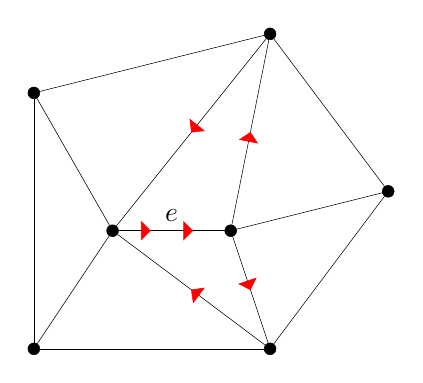
\begin{tikzpicture}
\begin{scope}[very thin,nodes={sloped,allow upside down}]     	\tikzset{
  arrow/.pic={\path[tips,every arrow/.try,->,>=#1] (0,0) -- +(.1pt,0);},
  pics/arrow/.default={triangle 90}}
      \tikzset{enclosed/.style={draw, circle, inner sep=0pt, minimum size=.15cm, fill=black}}

      \node[enclosed] (A) at (0,3.25) {};
      \node[enclosed] (B) at (3,4) {};
      \node[enclosed] (C) at (4.5,2) {};
      \node[enclosed] (D) at (3,0) {};
      \node[enclosed] (E) at (1,1.5) {};
      \node[enclosed] (F) at (2.5,1.5) {};
      \node[enclosed] (G) at (0,0) {};

	\draw (A) -- (E){};
	\draw (E) -- pic[pos=.3, red]{arrow} pic[pos=.7, red]{arrow}(F) node[midway, above]  {$e$};
	\draw (A) -- (B){};
	\draw (A) -- (G){};
	\draw (B) --pic[red]{arrow} (E){};
	\draw (F) --pic[red]{arrow} (B){};
	\draw (G) -- (E){};
	\draw (G) -- (D){};
	\draw (D) --pic[red]{arrow} (E){};
	\draw (F) --pic[red]{arrow} (D){};
	\draw (D) -- (C){};
	\draw (C) -- (F){};
	\draw (B) -- (C){};
\end{scope}
\end{tikzpicture}
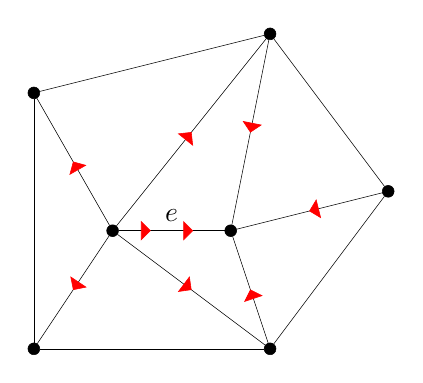
\begin{tikzpicture}
\begin{scope}[very thin,nodes={sloped,allow upside down}]     	\tikzset{
  arrow/.pic={\path[tips,every arrow/.try,->,>=#1] (0,0) -- +(.1pt,0);},
  pics/arrow/.default={triangle 90}}
      \tikzset{enclosed/.style={draw, circle, inner sep=0pt, minimum size=.15cm, fill=black}}

      \node[enclosed] (A) at (0,3.25) {};
      \node[enclosed] (B) at (3,4) {};
      \node[enclosed] (C) at (4.5,2) {};
      \node[enclosed] (D) at (3,0) {};
      \node[enclosed] (E) at (1,1.5) {};
      \node[enclosed] (F) at (2.5,1.5) {};
      \node[enclosed] (G) at (0,0) {};

	\draw (E) -- pic[red]{arrow}(A){};
	\draw (E) -- pic[pos=.3, red]{arrow} pic[pos=.7, red]{arrow}(F) node[midway, above]  {$e$};
	\draw (A) -- (B){};
	\draw (A) -- (G){};
	\draw (E) --pic[red]{arrow} (B){};
	\draw (B) --pic[red]{arrow} (F){};
	\draw (E) --pic[red]{arrow} (G){};
	\draw (G) -- (D){};
	\draw (E) --pic[red]{arrow} (D){};
	\draw (D) --pic[red]{arrow} (F){};
	\draw (D) -- (C){};
	\draw (C) --pic[red]{arrow} (F){};
	\draw (B) -- (C){};
\end{scope}
\end{tikzpicture}
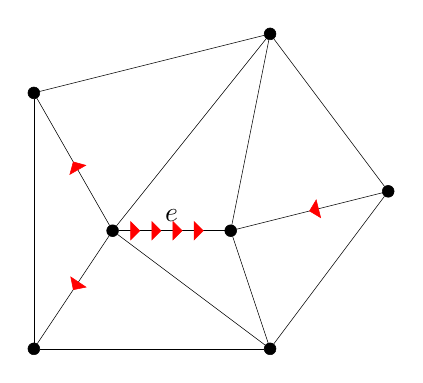
\begin{tikzpicture}
\begin{scope}[very thin,nodes={sloped,allow upside down}]     	\tikzset{
  arrow/.pic={\path[tips,every arrow/.try,->,>=#1] (0,0) -- +(.1pt,0);},
  pics/arrow/.default={triangle 90}}
      \tikzset{enclosed/.style={draw, circle, inner sep=0pt, minimum size=.15cm, fill=black}}

      \node[enclosed] (A) at (0,3.25) {};
      \node[enclosed] (B) at (3,4) {};
      \node[enclosed] (C) at (4.5,2) {};
      \node[enclosed] (D) at (3,0) {};
      \node[enclosed] (E) at (1,1.5) {};
      \node[enclosed] (F) at (2.5,1.5) {};
      \node[enclosed] (G) at (0,0) {};

	\draw (E) -- pic[red]{arrow}(A){};
	\draw (E) -- pic[pos=.2, red]{arrow} pic[pos=.4, red]{arrow} pic[pos=.6, red]{arrow} pic[pos=.8, red]{arrow}(F) node[midway, above]  {$e$};
	\draw (A) -- (B){};
	\draw (A) -- (G){};
	\draw (E) --(B){};
	\draw (B) -- (F){};
	\draw (E) --pic[red]{arrow} (G){};
	\draw (G) -- (D){};
	\draw (E) -- (D){};
	\draw (D) -- (F){};
	\draw (D) -- (C){};
	\draw (C) --pic[red]{arrow} (F){};
	\draw (B) -- (C){};
\end{scope}
\end{tikzpicture}
\end{figure}
\fi
Given $\sigma_1, \sigma_2$ two simplices in the basis  $ \beta_{n-1}$, we compute 
$$\langle \Delta \sigma_1, \sigma_2\rangle = \langle \partial^\star \sigma_1, \partial^\star \sigma_2\rangle + \langle \partial \sigma_1, \partial \sigma_2\rangle.$$
Note that for $j = 1,2$, there are exactly two $n$-dimensional simplices
$\tau^+_j, \tau^-_j$ containing $\sigma_j$ in their boundary and signs
$\varepsilon_j^+,\varepsilon_j^-\in \{-1,1\}$ such that 
$$
\partial^\star \sigma_j = \varepsilon_j^+\tau^+_j + \varepsilon_j^-\tau^-_j.
%\partial^\star \sigma_j = \tau^+_j - \tau^-_j.
$$
%They are oriented such that 
%Hence $\langle \partial \tau^{\pm}_j, \sigma_j \rangle = \pm 1$.
We distinguish four cases:
\begin{enumerate}
\item If $\sigma_1 = \sigma_2$, then $\tau_1^\pm = \tau_2^\pm$, $\varepsilon_1^{\pm}=\varepsilon_2^\pm$ and thus
  \begin{equation*}
    \langle \partial^\star \sigma_1, \partial^\star \sigma_2\rangle = \langle
    \varepsilon_1^+\tau^+_1 + \varepsilon_1^- \tau^-_1, \varepsilon_1^+\tau^+_1 + \varepsilon_1^-\tau^-_1 \rangle = 2.
  \end{equation*}
  On the other hand, $\partial \sigma_1$ consists of $n$ simplices of dimension $(n-2)$, hence 
$\langle \partial \sigma_1, \partial \sigma_2\rangle = n$ and we conclude
$$
\langle \Delta \sigma_1, \sigma_2 \rangle = n+2.
$$
\item
If $\sigma_1 \neq \sigma_2$ lie in the boundary of a common $n$-dimensional
simplex~$\tau$, up to replacing $\tau$ by $-\tau$ and exchanging the roles of $\tau_j^+$ and $\tau_j^-$, one can assume 
$$\tau = \tau_1^+ = \varepsilon \tau_2^+,$$
for some $\varepsilon \in \pm1$. Equivalently, the simplicial boundary of
$\tau$ contains $\sigma_1$ with sign $1$ and $\sigma_2$ with sign $\varepsilon$,
\begin{equation*}
  \langle \partial \tau,\sigma_1\rangle = 1;\quad \langle
  \partial\tau,\sigma_2\rangle = \varepsilon.
\end{equation*}
In particular we get
$$\langle \partial^\star \sigma_1, \partial^\star\sigma_2\rangle = \varepsilon.$$
%then up to {flipping} the orientation of $\sigma_1$ and/or that of $\sigma_2$, one can assume that $\tau^+_1 = \tau^{+}_2 = \tau$. In particular $\sigma_1$ and $\sigma_2$ both appear positively in $\partial \tau$, so that
%$$\langle \partial^\star \sigma_1, \partial^\star\sigma_2\rangle = +1.$$
As $n>1$ and we deal with a triangulation in this situation there is exactly one $(n-2)$-dimensional
simplex $\nu$ appearing in both $\partial \sigma_1$ and $\partial
\sigma_2$. We now claim that
$$
\langle \partial \sigma_1, \partial \sigma_2\rangle = -\varepsilon.
$$
To prove this, consider the simplicial chain
$0=\partial^2 \tau$. In the basis $\beta_{n-1}$ we have
\begin{equation*}
  \partial\tau = \sigma_1 + \varepsilon\sigma_2 + \sum_j \varepsilon_j\sigma_j
\end{equation*}
where the $\sigma_j$ are the faces of $\tau$ different of
$\sigma_1,\sigma_2$. Then $\langle\partial \sigma_j,\nu\rangle=0$ for those
$\sigma_j$ and
\begin{equation*}
 0 =\langle\partial^2\tau,\nu\rangle= \langle\partial\sigma_1+\varepsilon\partial\sigma_2,\nu\rangle
\end{equation*}
As $\nu$ is the only common term in the simplicial basis expansion of
$\partial\sigma_1$ and $\partial\sigma_2$ this implies indeed
$\langle\partial\sigma_1,\partial\sigma_2\rangle =-\varepsilon$.

Combining these computations we get
\begin{equation*}
  \langle \Delta \sigma_1, \sigma_2 \rangle
  =\langle\partial^*\sigma_1,\partial^*\sigma_2\rangle + \langle\partial\sigma_1,\partial\sigma_2\rangle = 0.
\end{equation*}
\item
If $\sigma_1$ and $\sigma_2$ share a common $(n-2)$-face, but are not in the boundary of a common $n$-dimensional simplex, then 
$\langle \partial^\star \sigma_1, \partial^\star \sigma_2 \rangle = 0$, and
$\langle \partial \sigma_1, \partial \sigma_2\rangle = \pm 1$. Moreover, if
$\sigma_1$ and $\sigma_2$ have compatible orientations, then by definition of
this notion $\langle \partial \sigma_1, \partial \sigma_2\rangle = -1$ and $\langle \partial \sigma_1, \partial \sigma_2\rangle =+1$ otherwise.
\item 
Finally, if $\sigma_1$ and $\sigma_2$ do not share a common face, then both $\langle \partial^\star \sigma_1, \partial^\star \sigma_2 \rangle$ and $\langle \partial \sigma_1, \partial \sigma_2 \rangle$ vanish.
\end{enumerate}
The proof is complete.
\end{proof}

\iffalse
\begin{definition}
\label{def:geod}
We say that a path along $(n-1)$-dimensional polyhedron of $\mathscr T$ is \emph{geodesic} if it satisfies the rule of the random walk, namely to consecutive simplices must be adjacent,
%with compatible orientation
and shall not bound a common $n$-simplex. A combinatorial closed geodesic path is a geodesic loop (or just a closed geodesic). 
%It is \emph{prime} if it cannot be written as t
\end{definition}
\fi


\begin{remark}\label{rem:generalize_trian}
 \cref{prop:Lapl} is the only property of the cell decomposition and resulting
 cellular Laplacian which is used in the following (together with Poincar\'e
 duality to identify the first and the codimension $1$ Betti numbers).

 We observe that the proof
 of \cref{prop:Lapl}
 works with slightly weaker conditions on the triangulation of our
 $n$-dimensional space: it suffices to
 have a decomposition into simplices such that each codimension $1$ simplex is
 in the boundary of exactly two $n$-dimensional simplices and such that each
 top dimensional simplex has exactly $(n+1)n/2$ distinct faces of codimension
 $2$, so that two codimension $1$ simplices intersect in at most one simplex
 of codimension $2$.

 Therefore, we can work with polyhedral decompositions into simplices which
 are not triangulations, as long as they satisfy these conditions.

 An example is illustrated in \cref{fig:torus}.
\end{remark}
\subsection{$L^2$-invariants}
\label{subsec:L2}
In this subsection, we consider the situation where the triangulation
defined in the previous subsection admits a free co-compact simplicial action of a group $\pi$. In this setting, we will denote by $\wh{\mathscr{T}}$ the triangulation, and by $\mathscr T = \wh{\mathscr{T}} / \pi$ the quotient, which we assume to be a triangulation of a compact manifold $M$ of dimension $n$. In other words, $\pi$ is a quotient of $\pi_1(M)$ and $\wh{\mathscr{T}}$ is a triangulation of the (in general non-compact) corresponding covering $\wh{M}$ of $M$.

The action of $\pi$ on $\wh{\mathscr{T}}$ gives the groups
$C_k(\wh{\mathscr{T}})_\ZZ$ the structure of free $\ZZ[\pi]$-modules of rank
$|\mathscr T^{(k)}| = \dim C_k(\mathscr T)$. The combinatorial Laplacian
$\Delta_k$ described in \cref{sec:lapl} acts on $C_k(\wh{\mathscr{T}})$ as a
$\pi$-equivariant operator, in the sense that
$$
\Delta_k (\alpha \cdot \hat \sigma) = \alpha \cdot \Delta_k \hat \sigma, \quad
\forall \hat \sigma \in C_k(\wh{\mathscr T}), \quad \forall\alpha \in \pi,
$$
and so does the transfer operator $T$ defined in \cref{prop:Lapl}. 
%Hence they induce matrices $\Delta^{(2)}_k \in  M({c_k},\ZZ[\pi])$ and $T^{(2)} \in M({c_{n-1}},\ZZ[\pi])$.
Note that any choice of lifts $\{\widehat{\sigma}_i^k\}$ of a finite basis $\{\sigma_i^k\}$ of $C_k({\mathscr T})$ yields a finite basis of $C_k(\wh{\mathscr T})_\ZZ$ as a free $\ZZ[\pi]$-module.

Complexifying, we obtain $C_k(\wh{\mathscr T})$ as a free $\mathbb C[\pi]$-module, yielding a complex vector space, generated by elements of the form
$$
\alpha \cdot \hat \sigma_i^k, \quad \alpha \in \pi, \quad i = 1, \dots, |\mathscr T^{(k)}|.
$$
We endow this space with a scalar product $\langle \cdot, \cdot \rangle_{L^2}$, defined by
\begin{equation}\label{eq:scalprod}
\left\langle \sum_{\alpha \in \pi} \lambda_\alpha \, \alpha\cdot\hat{\sigma}_i^k, \, \sum_{\beta\in \pi} \mu_{\beta} \, \beta \cdot \hat \sigma_j^k \right\rangle_{L^2} =  \delta_{i,j}\sum_{\alpha \in \pi} \lambda_\alpha \overline\mu_{\alpha^{-1}}.
\end{equation}
We will denote by $C_k^{(2)}(\mathscr T, \pi)$ the Hilbert space given by the completion of $C_k(\wh{\mathscr T})$ with respect to the norm induced by $\langle \cdot, \cdot \rangle_{L^2}$.

Given a bounded $\pi$-equivariant operator $P \colon C_k^{(2)}(\mathscr T, \pi) \to C_k^{(2)}(\mathscr T, \pi)$, we define its \emph{von Neumann trace} $\tr_{\mathrm{vN}}P$ by %It might be thought as follows: since $P$ is equivariant, it yields an operator on the finite dimensional quotient $C_k(\mathscr T)$, and $\tr_{\mathrm{vN}}(P)$ is just the trace of this matrix.\\
%More formally, it can be written as 
\begin{equation}
\label{eq:L2tracedef}
\tr_{\mathrm{vN}}P = \sum_{i=1}^{|\mathscr T^{(k)}|} \langle P\hat{\sigma}_i^k, \hat{\sigma}_i^k\rangle_{L^2}.
\end{equation}
Given any $\pi$-invariant closed subspace $U \subset C_k^{(2)}(\mathscr T, \pi)$, we define its \emph{von Neumann dimension} by
\begin{equation}
\label{eq:vNdim}
\dim_{\mathrm{vN}}U  = \tr_{\mathrm{vN}}\Pi_U,
\end{equation}
where $\Pi_U$ is the orthogonal projection on $U$.

The operator $\Delta_k$  induces a bounded, self-adjoint $\pi$-equivariant operator
\begin{equation*}
  \Delta^{(2)}_k \colon C_k^{(2)}(\mathscr T, \pi) \to C_k^{(2)}(\mathscr T, \pi).
\end{equation*}
It has real, non-negative,  bounded spectrum. The spectral theorem for bounded self-adjoint operators yields a family of orthogonal projections
$$
\left(E_k(\lambda)\right)_{\lambda \in \RR}; \quad E_k(\lambda)=\chi_{[0,\lambda]}(\Delta^{(2)}_k)
$$
 called the spectral family of $\Delta^{(2)}_k$ (\cite[Definition
 1.68]{Lueck}); it has the property that \(\displaystyle \Delta_k^{(2)} = \int_\RR \lambda \, dE_k(\lambda)\). Then the $L^2$-spectral density function of $\Delta_k^{(2)}$ is the function
\begin{equation}
\label{eq:SDF}
D_k \colon \RR \to \RR_{\geqslant 0}, \quad  \lambda \mapsto \tr_{\mathrm{vN}}  E_k(\lambda). 
 \end{equation}
By definition, the \emph{$k$-th $L^2$-Betti number $b_k^{(2)}(M, \pi)$} is the von Neumann dimension of $\ker \Delta^{(2)}_k$, so that $b_k^{(2)}(M, \pi) = D_k(0)$.

Because $\Delta^{(2)}_k$ is bounded, for all $\lambda \geqslant \lVert \Delta^{(2)}_k\rVert$ the function $D_k$ is constant, equal to $D_k(\lambda)=|\mathscr T^{(k)}|$.

\begin{definition}
\label{def:detclass}
The Laplacian $\Delta_k^{(2)}$ is said to be \emph{of determinant class} if the Stieltjes integral
\begin{equation}
\label{eq:FKdef}
\int_{0^+}^\infty \log \lambda \, \dd D_k(\lambda) =
\lim_{\substack{\varepsilon \to 0\\ \varepsilon >0 }}
\int_{\varepsilon}^\infty \log \lambda \, \dd D_k(\lambda) \in \mathbb{R}
\end{equation}
exists as a real number, and in this case the \emph{Fuglede--Kadison determinant} of $\Delta_k^{(2)}$ is given by
$$
{\det}_{\mathrm{FK}}(\Delta_k^{(2)}) = \exp\int_{0^+}^\infty \log \lambda \,
\dd D_k(\lambda) \in (0,\infty).
$$
\end{definition}

%\newpage 

\begin{remark}
  \strut
  \begin{itemize}
  \item The definition of Fuglede--Kadison determinant generalizes of course
    in the same way to any non-negative Hilbert $\vN\pi$-module endomorphism
    $A\colon U\to U$ (with $\dim_{\vN}(U)<\infty$), see \cite[Chapter 3]{Lueck}.
\item
The integrals on the right-hand side of \cref{eq:FKdef} are finite: the
boundedness of $\Delta^{(2)}_k$ implies that they are indeed integrals on
$[\varepsilon, \lVert \Delta^{(2)}_k\rVert]$.
\item By definition, if $\log(A)$ is defined by spectral calculus, i.e.~if
  $\sigma(A)\subset (0,\infty),$ then
  \begin{equation*}
    \log\detFK(A) = \tr_{\vN}(\log(A)) \quad\implies \quad\detFK(A)= \exp(\tr_{\vN}(\log(A))).
  \end{equation*}
\item In case the group $\pi$ is finite, i.e.~if
  we deal with a finite cover $\widehat M$ of $M$, then the FK-determinant
  is nothing but the 
  usual determinant of the positive matrix $\Delta^{(2)}_k$ restricted to the
  orthogonal of its kernel (i.e.~the product of the non-zero eigenvalues), but
  then raised to the power $1/|\pi|$.
\end{itemize}
\end{remark}
% From the definition of the Fuglede--Kadison determinant, it follows that if a self-adjoint operator $P \colon C_{k}^{(2)}(\mathscr T, \pi) \to C_{k}^{(2)}(\mathscr T, \pi)$ is of determinant class, so is $\nu P$ for any $\nu > 0$, and
% \begin{equation}\label{eq:dethom}
% {\det}_{\mathrm{FK}} (\nu P) = \nu^{c_k}\, {\det}_{\mathrm{FK}} P.
% \end{equation}
% This follows from the fact that the spectral family of $\nu P$ is $(E(\lambda/\nu))_{\lambda \in \mathbb R}$ if $(E(\lambda))_{\lambda \in \mathbb R}$ is the spectral family of $P$.


Later, we will use the following basic properties of the Fuglede--Kadison
determinant.
By \cite[Lemma 3.15
    (7)]{Lueck} we have 
  \begin{equation}\label{item:add}
    {\det}_{\mathrm{FK}}(A\oplus B) =
    {\det}_{\mathrm{FK}}(A)\cdot {\det}_{\mathrm{FK}}(B) .
  \end{equation}
 If $\lambda\in (0,\infty)$
    and $A\colon U\to U$ is an injective endomorphism of the Hilbert
    $\mathcal{N}\left(\pi\right)$-module $U$ of finite von Neumann dimension then
    \begin{equation}\label{item:mult} 
      {\det}_{\mathrm{FK}}(\lambda A) =
      \lambda^{\dim_{\vN}(U)}{\det}_{\mathrm{FK}}(A)
    \end{equation}
    by \cite[Theorem 3.14 (1) and (6)]{Lueck}.

    We also need the following continuity result for the Fuglede--Kadison
determinant, which is not 
explicitly treated in \cite[Chapter 3]{Lueck}.
\begin{lemma}\label{lem:FK}
  Let $A\colon U\to U$ be a positive injective Hilbert $\vN\pi$-module endomorphism where
  $\dim_{\vN}(U)<\infty$.
  Then $f(z)=z\mapsto \detFK(A+z\Id)$ is an analytic function defined on
  $(0,\infty)$. It extends continuously at $0$ with
  \begin{equation}\label{item:conv}
    \lim_{z\to 0^+} f(z) = \detFK(A).
  \end{equation}
  If $A$ is not of determinant class and hence $\detFK(A)=0$, then $f(z)$
  converges to $0$ for $z\to 0$ slower than any positive power of $z$. More
  precisely, for
  every $C>0$ and $\alpha>0$, there exists $\varepsilon>0$ such that
  \begin{equation*}
    f(z) > C z^\alpha,\qquad  z\in(0,\varepsilon).
  \end{equation*}
\end{lemma}
\begin{proof}
  Let $F(t)=\tr_{\vN}(\chi_{[0,t]}(A))$ be the spectral density function of
  $A$ (using measurable functional calculus with the characteristic function
  $\chi_{[0,t]}$ of the interval $[0,t]\subset\RR$).

  Then by the proof of \cite[Lemma 3.15 (5)]{Lueck} we have
  \begin{equation*}
    \detFK(A+z\Id) = \int_{0^+}^{\norm{A}} \log(\lambda+z)\,dF(\lambda).
\end{equation*}
Around each $z_0>0$, the function $z\mapsto \log(\lambda+z)$ has an absolutely
convergent power series expansion, with convergence uniform in $\lambda\in
[0,\norm{A}]$. Therefore,  
$\detFK(A+z\Id)$ is also analytic on $(0,\infty)$ by the continuity of the Stieltjes integral.

The continuity at $0$ is established in \cite[Lemma 3.15 (5)]{Lueck} with
$\lim_{\varepsilon\to 0^+}    {\det}_{\mathrm{FK}}(A+\varepsilon\Id)
={\det}_{\mathrm{FK}}(A)$.
  
Finally, to control the behaviour of $f$ near $0$, choose $C>0$ and
$\alpha>0$. On $(0,C^{-1/\alpha})$ we have $C\leqslant z^{-\alpha}$ and hence
$z^{\alpha}\geqslant C z^{2\alpha}$. Therefore, it suffices to find $\varepsilon>0$
such that $f(z)>z^\alpha$ on $(0,\varepsilon)$ to conclude the proof.

Now, we use that the spectral density function $F$ is right continuous and
increasing. Set ${\nu}=\frac{\alpha}{2\dim_{\vN}(U)}$. As $F(0)=0$ by the
injectivity of $A$, we can choose 
$\varepsilon>0$ such that $F(z^{\nu})<\frac{\alpha}{2}$ whenever $z<\varepsilon$.

With this $\varepsilon$ which we choose smaller than $1$ and for $0<z<\varepsilon<1$ we then have
\begin{equation*}
  \begin{split}
    \int_{0}^{\norm{A}} \log(\lambda+z)\,dF(\lambda) 
& = \int_0^{z^{\nu}}\log(\lambda+z)\,dF(\lambda)+\int_{z^{\nu}}^{\norm{A}}
  \log(\lambda+z)\,dF(\lambda)\\
  & \geqslant \int_0^{z^{\nu}}\log(z)\,dF(\lambda) +\int_{z^{\nu}}^{\norm{A}}
    \log(z^{\nu}+z)\,dF(\lambda)\\
&\geqslant F(z^{\nu})\log(z) + (\underbrace{F(\norm{A})}_{=\dim_{\vN}(U)}-F(z^{\nu})) \log(z^{\nu})\\
    & {\geqslant } \frac{\alpha}{2} \log(z) +
      \dim_{\vN}(U){\nu}\log(z)\\
    &{=} \alpha \log(z),
  \end{split}
\end{equation*}
where we used $\log(z)<0$ for $z < 1$ in the last inequality and $\nu = \alpha / (2 \dim_{\mathrm{vN}}(U))$ in the last equality.
Consequently, for $0<z<\varepsilon$ as chosen above,
\begin{equation*}
  \begin{split}
    \detFK(A+z\Id) & = \exp\left(\int_0^{\norm{A}} \log(\lambda+z)\,dF(\lambda)
                     \right)\\
    & \geqslant \exp(\alpha\log(z)) = z^\alpha.
  \end{split}
\end{equation*}
This completes the proof.
\end{proof}


\section{First Betti number and combinatorial Ruelle zeta function}
\label{sec:fried}
%Let $K$ be a fixed oriented triangulation of $\Sigma$, and let $K^*$ denote the dual complex: it is a CW-complex consisting of one vertex for each triangle in $K$, one edge joining each pair of such vertices provided they correspond to adjacent faces (hence edges of $K^*$ are in 1:1 correspondence with edges of $K$), and one face for each vertex of $K$. The orientations are prescribed as follows: the Hodge star rotates edges in the direct sense (see \cref{fig:K}), and maps a vertex with positive sign onto its dual face positively oriented.
%
%
%Of course, faces of the complex $K^*$ are not triangles in general (except if one started with a regular triangulation of degree 3).
%
%The induced map $\star \colon C_*(K) \to C_*(K^*)$ is the Hodge star. We define the co-boundary operator $\partial^\star = \star \partial \star \colon C_*(K) \to C_{*+1}(K)$, and the combinatorial Laplacian $\Delta = \partial\partial^\star + \partial^\star\partial$.
%
%An explicit local computation (see \cref{fig:2}) shows the following:
%\begin{proposition} \label{prop:Lapl}
%The Laplacian operator writes
%\begin{equation}
%\label{eq:transfer}
%\Delta = 4 \Id - T
%\end{equation}
%
%where $T$ is a symmetric matrix whose entries are 
%\begin{itemize}
%\item $T_{ij}= 0$ if $i=j$ or $i$ and $j$ does not share a vertex, or are adjacent to the same triangle
%\item $T_{ij}= 1$ if $i$ and $j$ share a vertex with compatible orientation, and do not belong to the same triangle
%\item $T_{ij}= -1$ if $i$ and $j$ share a vertex with opposite orientation, and do not belong to the same triangle.
%\end{itemize}
%\end{proposition}

%\begin{figure}[h]
%\caption{\label{fig:2} Computations of $d\delta e$ (up on the left) and of $\delta d e$ (up on the right). We summarize with $\Delta e$ (below).}
%\begin{tikzpicture}
%\begin{scope}[very thin,nodes={sloped,allow upside down}]     	\tikzset{
%  arrow/.pic={\path[tips,every arrow/.try,->,>=#1] (0,0) -- +(.1pt,0);},
%  pics/arrow/.default={triangle 90}}
%      \tikzset{enclosed/.style={draw, circle, inner sep=0pt, minimum size=.15cm, fill=black}}
%
%      \node[enclosed] (A) at (0,3.25) {};
%      \node[enclosed] (B) at (3,4) {};
%      \node[enclosed] (C) at (4.5,2) {};
%      \node[enclosed] (D) at (3,0) {};
%      \node[enclosed] (E) at (1,1.5) {};
%      \node[enclosed] (F) at (2.5,1.5) {};
%      \node[enclosed] (G) at (0,0) {};
%
%	\draw (A) -- (E){};
%	\draw (E) -- pic[pos=.3, red]{arrow} pic[pos=.7, red]{arrow}(F) node[midway, above]  {$e$};
%	\draw (A) -- (B){};
%	\draw (A) -- (G){};
%	\draw (B) --pic[red]{arrow} (E){};
%	\draw (F) --pic[red]{arrow} (B){};
%	\draw (G) -- (E){};
%	\draw (G) -- (D){};
%	\draw (D) --pic[red]{arrow} (E){};
%	\draw (F) --pic[red]{arrow} (D){};
%	\draw (D) -- (C){};
%	\draw (C) -- (F){};
%	\draw (B) -- (C){};
%\end{scope}
%\end{tikzpicture}
%\begin{tikzpicture}
%\begin{scope}[very thin,nodes={sloped,allow upside down}]     	\tikzset{
%  arrow/.pic={\path[tips,every arrow/.try,->,>=#1] (0,0) -- +(.1pt,0);},
%  pics/arrow/.default={triangle 90}}
%      \tikzset{enclosed/.style={draw, circle, inner sep=0pt, minimum size=.15cm, fill=black}}
%
%      \node[enclosed] (A) at (0,3.25) {};
%      \node[enclosed] (B) at (3,4) {};
%      \node[enclosed] (C) at (4.5,2) {};
%      \node[enclosed] (D) at (3,0) {};
%      \node[enclosed] (E) at (1,1.5) {};
%      \node[enclosed] (F) at (2.5,1.5) {};
%      \node[enclosed] (G) at (0,0) {};
%
%	\draw (E) -- pic[red]{arrow}(A){};
%	\draw (E) -- pic[pos=.3, red]{arrow} pic[pos=.7, red]{arrow}(F) node[midway, above]  {$e$};
%	\draw (A) -- (B){};
%	\draw (A) -- (G){};
%	\draw (E) --pic[red]{arrow} (B){};
%	\draw (B) --pic[red]{arrow} (F){};
%	\draw (E) --pic[red]{arrow} (G){};
%	\draw (G) -- (D){};
%	\draw (E) --pic[red]{arrow} (D){};
%	\draw (D) --pic[red]{arrow} (F){};
%	\draw (D) -- (C){};
%	\draw (C) --pic[red]{arrow} (F){};
%	\draw (B) -- (C){};
%\end{scope}
%\end{tikzpicture}
%\begin{tikzpicture}
%\begin{scope}[very thin,nodes={sloped,allow upside down}]     	\tikzset{
%  arrow/.pic={\path[tips,every arrow/.try,->,>=#1] (0,0) -- +(.1pt,0);},
%  pics/arrow/.default={triangle 90}}
%      \tikzset{enclosed/.style={draw, circle, inner sep=0pt, minimum size=.15cm, fill=black}}
%
%      \node[enclosed] (A) at (0,3.25) {};
%      \node[enclosed] (B) at (3,4) {};
%      \node[enclosed] (C) at (4.5,2) {};
%      \node[enclosed] (D) at (3,0) {};
%      \node[enclosed] (E) at (1,1.5) {};
%      \node[enclosed] (F) at (2.5,1.5) {};
%      \node[enclosed] (G) at (0,0) {};
%
%	\draw (E) -- pic[red]{arrow}(A){};
%	\draw (E) -- pic[pos=.2, red]{arrow} pic[pos=.4, red]{arrow} pic[pos=.6, red]{arrow} pic[pos=.8, red]{arrow}(F) node[midway, above]  {$e$};
%	\draw (A) -- (B){};
%	\draw (A) -- (G){};
%	\draw (E) --(B){};
%	\draw (B) -- (F){};
%	\draw (E) --pic[red]{arrow} (G){};
%	\draw (G) -- (D){};
%	\draw (E) -- (D){};
%	\draw (D) -- (F){};
%	\draw (D) -- (C){};
%	\draw (C) --pic[red]{arrow} (F){};
%	\draw (B) -- (C){};
%\end{scope}
%\end{tikzpicture}
%\end{figure}
\subsection{The compact case}
The purpose of this paragraph is to prove \cref{theo:mainfried}.

\medbreak

Let us fix a compact oriented manifold $M$ of dimension $n>1$ with a triangulation~$\mathscr T$. %We assume $\mathscr T$ is regular: that any $(n-1)$-dimensional polyhedron in $\mathscr T$ has exactly $N$ hyperfaces in its boundary.

\begin{definition}\label{def:reversing_ind}
For a combinatorial closed geodesic $\gamma$, we denote by $n_\gamma$ the
\textit{reversing number} of $\gamma$, that is, the number of adjacent pairs
with non-compatible orientation (as defined in Definition \ref{def:compa})
appearing in $\gamma$. Its parity 
$$
\varepsilon_\gamma = (-1)^{n_\gamma}
$$
is called the \textit{reversing index} of $\gamma$.
\end{definition}

For an illustration of this concept, see \cref{fig:sign}.

\begin{figure}[h]
\caption{\label{fig:sign} Some closed primitive unmarked geodesics $\gamma_i, \, i=1 \ldots 4,$ from left to right. The extra edges are browsed twice (back-and-forth). For the first one on the left, $n_{\gamma_1} = 0$, then $n_{\gamma_2}=1$ and $n_{\gamma_3} = n_{\gamma_4} = 2$.}
\begin{tikzpicture} 
%% vertices
\draw[fill=black] (-3,0) circle (1pt);
\draw[fill=black] (-2,0) circle (1pt);
\draw[fill=black] (-2,1) circle (1pt);
\draw[fill=black] (-3,1) circle (1pt);
%%% edges
\draw[-Stealth] (-3,0) -- (-2.5,0);
\draw[-Stealth] (-2,0) -- (-2,0.5);
\draw[-Stealth] (-2,1) -- (-2.5,1);
\draw[-Stealth] (-3,1) -- (-3,0.5);
\draw (-2.5,0) -- (-2,0);
\draw (-2,0.5) -- (-2,1);
\draw (-2.5,1) -- (-3,1);
\draw (-3,0.5) -- (-3,0);

 %% vertices
\draw[fill=black] (0,0) circle (1pt);
\draw[fill=black] (1,0) circle (1pt);
\draw[fill=black] (1,1) circle (1pt);
\draw[fill=black] (0,1) circle (1pt);
\draw[fill=black] (-0.4,-0.4) circle (1pt);
%%% edges
\draw[-Stealth] (0,0) -- (0.5,0);
\draw[-Stealth] (1,0) -- (1,0.5);
\draw[-Stealth] (1,1) -- (0.5,1);
\draw[-Stealth] (0,1) -- (0,0.5);
\draw[-Stealth] (-0.4,-0.4) -- (-0.15, -0.15);
\draw (0.5,0) -- (1,0);
\draw (1,0.5) -- (1,1);
\draw (0.5,1) -- (0,1);
\draw (0,0.5) -- (0,0);
\draw (-0.15, -0.15) -- (0,0);

 %% vertices
\draw[fill=black] (3,0) circle (1pt);
\draw[fill=black] (4,0) circle (1pt);
\draw[fill=black] (4,1) circle (1pt);
\draw[fill=black] (3,1) circle (1pt);
\draw[fill=black] (2.6,-0.4) circle (1pt);
\draw[fill=black] (4.4,1.4) circle (1pt);

%%% edges
\draw[-Stealth] (3,0) -- (3.5,0);
\draw[-Stealth] (4,0) -- (4,0.5);
\draw[-Stealth] (4,1) -- (3.5,1);
\draw[-Stealth] (3,1) -- (3,0.5);
\draw[-Stealth] (2.6,-0.4) -- (2.85, -0.15);
\draw[-Stealth] (4,1) -- (4.25, 1.25);
\draw (3.5,0) -- (4,0);
\draw (4,0.5) -- (4,1);
\draw (3.5,1) -- (3,1);
\draw (3,0.5) -- (3,0);
\draw (2.85, -0.15) -- (3,0);
\draw (4.25, 1.25) -- (4.4,1.4);

 %% vertices
\draw[fill=black] (6,0) circle (1pt);
\draw[fill=black] (7,0) circle (1pt);
\draw[fill=black] (7,1) circle (1pt);
\draw[fill=black] (6,1) circle (1pt);

%%% edges
\draw[-Stealth] (6,0) -- (6.5,0);
\draw[-Stealth] (7,0) -- (7,0.5);
\draw[arrows = {-Stealth[reversed]}] (7,1) -- (6.5,1);
\draw[-Stealth] (6,1) -- (6,0.5);
\draw (6.5,0) -- (7,0);
\draw (7,0.5) -- (7,1);
\draw (6.5,1) -- (6,1);
\draw (6,0.5) -- (6,0);
\end{tikzpicture}

\end{figure}
%\fi
%We also denote by $n_k$ the number of marked geodesic loops (non-necessarily prime) of length. 

\begin{definition}
  For any combinatorial closed geodesic $\gamma$, we denote by $\gamma^\sharp$
  the unique primitive combinatorial closed geodesic so that $\gamma$ is a power of $\gamma^\sharp$. Recall that $|\gamma^\sharp|$ denotes the length of $\gamma^\sharp$.
%\iffalse
\end{definition}

\begin{lemma}
\label{prop:trace}
For each $k = 1, 2, \dots$, it holds
\begin{equation}
\label{eq:transfer}
\tr T^k = 
%n_k = 
\sum_{|\gamma| = k} \varepsilon_\gamma |\gamma^\sharp|,
\end{equation}
where the sum runs over all combinatorial closed geodesics (not necessary primitive).
\end{lemma}
%\begin{remark}
%Here we forbid closed geodesics going through two consecutive edges in a triangle, but we allow backtracks. In particular, we see that $n_2=2|E|$ is twice the number of edges of the triangulation. Note that $n_3=0$.
%\end{remark}
\begin{proof}
By the rules for the product of matrices, for $\sigma \in  \beta_{n-1}$ the
diagonal coefficient $(T^k)_{\sigma,\sigma}$ of the k-th power of $T$ at
$\sigma$ is given as
$$
(T^k)_{\sigma, \sigma}= \sum_{\sigma_1, \ldots, \sigma_{k-1}} T_{\sigma, \sigma_1}T_{\sigma_1, \sigma_2} \ldots T_{\sigma_{k-1}, \sigma}
$$
where a priori the $\sigma_j$ run through the basis $\beta_{n-1}$. But of
course, we can restrict to those tuples where none of the terms
$T_{\sigma_j,\sigma_{j+1}}$ is zero. By \cref{prop:Lapl}, this means
  that the sum is over all tuples forming an admissible path
  $(\sigma,\sigma_1,\dots,\sigma_{k-1},\sigma)$. Moreover, by 
  \cref{prop:Lapl} and \cref{def:reversing_ind} of the reversing
  index $\varepsilon_\gamma$, we have 
$$
T_{\sigma, \sigma_1}T_{\sigma_1, \sigma_2} \ldots T_{\sigma_{k-1}, \sigma} = \varepsilon_\gamma
$$
whenever $\gamma$ is represented by the combinatorial closed geodesic
$(\sigma, \sigma_1, \dots, \sigma_{k-1})$. Finally, each combinatorial closed geodesic
$\gamma$ will appear exactly $|\gamma^\sharp|$ times in $\tr T^k$, which
concludes the proof.
\end{proof}

With this trace formula in hand, let us prove \cref{theo:mainfried}, which we recall here. The transfer matrix $T$ is defined in \cref{prop:Lapl}.
\begin{theorem}\label{theo:fried}
Let $\rho(T)$ be the spectral radius of the transfer matrix $T$. Then for $|z|<\rho(T)^{-1}$ we have
\begin{equation}\label{eq:zetaprod}
\zeta_{\mathscr T}(z) = \prod_{\gamma \in \mathcal{P}}\left(1-\varepsilon_\gamma z^{|\gamma|}\right) = \det\left(\mathrm{Id} - z T\right).
\end{equation}
In particular, $\zeta_{\mathscr T}(z)$ extends to a polynomial function
defined on the whole complex plane $\CC$. 
Moreover, it has a zero of order $b_1(M)$ at $z=(n+2)^{-1}$.
\end{theorem}


\begin{proof}
Using that for a positive complex matrix $\log(\det(A))=\tr(\log(A))$ and
using the power series of $\log$, we have
$$
\begin{aligned}
\det(\mathrm{Id} - zT) &= \exp \left(- \sum_{k=1}^\infty \frac{z^k}{k} \tr T^k
\right)&= \exp\left( - \sum_{k = 1}^\infty \frac{z^k}{k} \sum_{|\gamma| = k} \varepsilon_\gamma |\gamma^\sharp|\right).
\end{aligned}
$$
This makes sense for $z\in\CC$ with $|z|<\rho(T)^{-1}$ because then $\lVert
zT\rVert <1$, hence  $\mathrm{Id}-zT$ is positive and the series converge absolutely. 

Now we have
\begin{equation*}
{\sum_{|\gamma| = k} \varepsilon_\gamma |\gamma^\sharp| = \sum_{\gamma \in \mathcal P} |\gamma|\sum_{p\in\mathbb{N}:~p\cdot|\gamma| = k}\varepsilon_\gamma^p},
\end{equation*}
hence one gets
$$
\begin{aligned}
\det(\mathrm{Id} - zT) &= \exp \left(- \sum_{\gamma \in \mathcal P} |\gamma| \sum_{p=1}^\infty\frac{z^{p|\gamma|}}{p|\gamma|} \varepsilon_\gamma^p\right) \\
&= \prod_{\gamma \in \mathcal P} \exp \left(- \sum_p \frac{\left(\varepsilon_\gamma z^{|\gamma|}\right)^p}{p}\right),
\end{aligned}
$$
which proves \cref{eq:zetaprod}. Finally, by \cref{prop:Lapl}, we have
\begin{equation*}
  \begin{split}
    \det\left(\mathrm{Id}-(z-\frac{1}{2+n})T\right) &= \det\left( \mathrm{Id}
                                                      -(z-\frac{1}{2+n})
                                                      ((n+2)\mathrm{Id}-\Delta)\right) \\
    &=  \det\left(\frac{1}{2+n}\Delta+ z (\Delta-(n+2))  \right)
  \end{split}
\end{equation*}
which vanishes at zero of order $\dim\ker(\Delta_{n-1})$, as we see by
diagonalizing $\Delta_{n-1}$.
% $$
% \det(\mathrm{Id} - zT) = z^{\dim C_{n-1}(\mathscr T)} \det\left(\frac{1 - z\, (n+2)}{z} \mathrm{Id} + \Delta_{n-1} \right)
% $$
% where $\Delta_{n-1}  = \Delta|_{C_{n-1}(\mathscr T)}$. However
Moreover, by a standard linear algebra/functional analysis result (sometimes
called finite 
dimensional Hodge theory, see~\cite[Appendix A]{nicolaescu2008reidemeister} for an exposition of this circle of ideas), we have
$$\ker(\partial) = \im(\partial)\oplus \ker(\Delta)\quad\implies \;\dim \ker \Delta_{n-1} = b_{n-1}(M).$$
Finally by Poincar\'e duality $b_{n-1}(M)=b_1(M)$ and we conclude that
$\det(\mathrm{Id} - zT)$ vanishes of order $b_1(M)$ at $z = (n+2)^{-1}$.
%This completes the proof.
%Using \eqref{eq:transfer}, for $\Re(z)$ big enough one writes
%\begin{eqnarray*}
%\det(\Delta_{C^1}+z)&=&\det(4\Id-T+z)\\
%&=&(4+z)^{\vert E\vert}\det(\Id- (4\Id+z)^{-1} T)\\
%&=&(4+z)^{\vert E\vert}\exp\left(\tr\log (\Id- (4\Id+z)^{-1} T)\right)\\
%&=&(4+z)^{\vert E\vert}\exp\left( \sum_{k=1}^\infty (4+z)^{-k} \frac{\tr(  T^k)
%}{k}\right)\\
%&=&(4+z)^{\vert E\vert}\exp\left( \sum_{k=1}^\infty (4+z)^{-k} \frac{n_k
%}{k}\right).
%\end{eqnarray*}
%Now the first term $(4+z)^{\vert E\vert}$ does not vanish at $z=0$, hence the function  $\exp\left( \sum_{k=1}^\infty (4+z)^{-k} \frac{n_k}{k}\right)$ vanishes at $z=0$ at order $b_1(\Sigma)$.
%It proves the theorem.
\end{proof}

We now give the short proof of \cref{corol:2_and_4_mf}.
\begin{proof}[Proof of \cref{corol:2_and_4_mf}]
  For a compact connected orientable surface $F$, the Euler characteristic
  satisfies $\chi(F)=2-b_1(F)$ and we have
  $n=2$, hence by \cref{corol:1stBetti} the combinatorial closed geodesics of length
  bounded by the number of edges in the triangulation and their reversing
  indices determines $\chi(F)$.

  If $M$ is a compact connected oriented manifold with $\dim(M)\leqslant 4$ we know
  a priori that $b_0(M)=b_4(M)=1$ and by \cref{corol:1stBetti} we determine
  $b_1(M)=b_3(M)$. Finally, $b_2(M)=\chi(M)-2+b_1(M)+b_3(M)$ is now determined
  by the Euler characteristic which can be read of from the combinatorial data
  of the triangulation (namely the number of simplices of different dimension).
\end{proof}
\subsection{The non-compact case: $L^2$-Betti numbers}
In this section we consider the setting of \cref{subsec:L2}: the compact
manifold $M$ with triangulation $\mathscr T$ comes with a normal covering
$\wh{M}$ with free action by a quotient $\pi$ of the fundamental group $\pi_1(M)$. The triangulation $\mathscr T$ lifts as $\wh{\mathscr{T}}$, for which we fix a basis $\{\hat{\sigma}^{n-1}_i\}_{i=1, \ldots |\mathscr T^{(n-1)}|}$ for the space $C_{n-1}(\wh{\mathscr{T}})$ as $\ZZ[\pi]$-module.

We denote by $\wh{\mathcal P}$ the set of primitive combinatorial closed geodesics in $\wh{\mathscr{T}}$ starting from one of the $\hat{\sigma}^{n-1}_i$.
Recall that $T$ is the transfer operator associated to the geodesic random walk on $\wh{\mathscr T}$ described in \cref{prop:Lapl}.

Then \cref{prop:trace} holds true in this setting, namely:
\begin{lemma}
\label{prop:L2trace}
For each $k = 1, 2, \dots$, it holds
\begin{equation}
\label{eq:transferL2}
\tr_{\mathrm{vN}} T^k = 
%n_k = 
\sum_{|\gamma| = k} \varepsilon_\gamma |\gamma^\sharp|,
\end{equation}
where the sum runs over all combinatorial closed geodesics (not necessary primitive) which start at one of the $\hat{\sigma}^{n-1}_i$.
\end{lemma}
\begin{proof}
Using the definition of the von Neumann trace given in \cref{eq:L2tracedef}, the proof is exactly the same as for \cref{prop:trace}.
\end{proof}

Now we prove \cref{theo:mainL2}, which we recall here:
\begin{theorem}
The function 
\begin{equation}
\label{zeta}
\zeta^{(2)}_{\wh{\mathscr T}}(z) = \prod_{\gamma \in \widehat{\mathcal P}} (1- \varepsilon_\gamma z^{|\gamma|})
\end{equation}
converges for $|z| \ll 1$, and has an analytic extension to the disk of diameter $(0, \frac 1 {n+2})$. Moreover,
$$
\zeta^{(2)}_{\wh{\mathscr T}}\left(\frac{1}{n+2}-z\right) = z^{b_1^{(2)}(M,\pi)} f(z) 
$$
with a function $f$ which is continuous at $0$.  If $\Delta_{n-1}^{(2)}$ is of
determinant class, then
\begin{equation*}
  f(0) =(n+2)^{2b_1^{(2)}(M,\pi)-|\mathscr T^{(n-1)}|} \cdot \detFK(\Delta_{n-1}^{(2)}).
\end{equation*}
If $\Delta_{n-1}^{(2)}$ is not of determinant class, then $f(0)=0$ but $f$
converges slower to $0$ than any power of $z$ in the sense that for all $C>0$,
$\alpha>0$ there is $\varepsilon>0$ such that
\begin{equation*}
  f(z)> Cz^\alpha\qquad\forall 0<z<\varepsilon.
\end{equation*}
In particular, the function $\zeta^{(2)}_{\wh{\mathscr T}}$ and hence the
combinatorial closed geodesics on $\widehat M$ together with the data of
$|\mathscr T^{(n-1)}|$ determine $b_{n-1}^{(2)}(M, \pi)$.
%then its value as $z = \frac 1 {n+2}$ is well defined: it vanishes at order $b_{n-1}^{(2)}(M)$, and is equal to $\det_{L^2}(\Delta_{n-1}^{(2)})$ when $b_{n-1}^{(2)}(M)$ vanishes.
\end{theorem}

\begin{remark}
  The term $\det_{FK}(\Delta^{(2)}_{n-1})$ appearing in \cref{theo:mainL2} is
  a very delicate spectral invariant which highly depends on the specific
  triangulation and is not a topological invariant (only the property of being
  of determinant class is a topological invariant, even a homotopy invariant,
  of the manifold $M$). We therefore don't assign too much meaning to it.

  Note, however, that a combination of the Fuglede--Kadison determinants of
  all the combinatorial $L^2$-Laplacians gives the $L^2$-torsion of $M$, a
  very interesting topological invariant, compare \cite[Chapter 3]{Lueck}. This is similar to the compact Riemannian case, it is well--known that the Ray--Singer zeta determinant of the Laplacian acting on functions is not a topological invariant. However, a combination of the zeta determinants for the Laplacian acting on forms of all degrees gives the analytic torsion which happens to be a topological invariant.   
   A
  case of interest to us are closed 3-manifolds. Here,
  the $L^2$-torsion (of the universal covering) is proportional to the sum of
  the volumes of the hyperbolic pieces in the JSJ-decomposition by
  \cite{LueckSchick}. 
\end{remark}

\begin{proof}
Since the triangulation $\wh{\mathscr T}$ is a lift of a triangulation of a
compact manifold, there is a global upper-bound $K$ on the number of neighbors
of any $n-1$ simplex, in particular there are less than $K^k$ primitive
combinatorial closed geodesics of length $k$. It follows that the infinite product \eqref{zeta} converges for $|z| < K^{-1}$.

Now using \cref{prop:L2trace} and functional calculus one sees that 
\begin{equation}
\label{eq:logdet}
{\det}_{\mathrm{FK}}(\Id - zT) = \exp\left(- \sum_{k=1}^\infty \frac{z^k}{k} \tr_{\vN} T^k
\right)
\end{equation}
on the real interval $\left]-\frac 1 K, \frac 1 K\right[$, since there the
operator $\log(\Id - zT)$ is well-defined and is given by the power series in
\cref{eq:logdet}. One deduces just as in the proof of \cref{theo:fried} that
$$\zeta^{(2)}_{\wh{\mathscr T}}(z) = {\det}_{\mathrm{FK}}(\Id - z T).$$


We will use \cref{item:add} for the orthogonal decomposition $\Id = p_K \oplus q_K$
with $p_K$ the orthogonal projection onto $\ker(\Delta^{(2)}_{n-1})$ and
$q_K=1-p_K$. This decomposition is preserved by $\Delta^{(2)}_{n-1}$ and
satisfies of course $\Delta_{n-1}^{(2)}p_K=0$, and that
$\Delta^{(2)}_{n-1}q_K$ is injective on $\im(q_K)$. Note also that by
definition, one has 
$$
\dim_{\vN}(\im(p_K)) = b_{n-1}^{(2)}(M,\pi) =
b_1^{(2)}(M,\pi).
$$

Note that from \cref{prop:Lapl} one has
\begin{equation*}
  T = (n+2)\Id - \Delta_{n-1}^{(2)},
\end{equation*}
hence we obtain
\begin{equation*}
  \begin{split}
    \zeta^{(2)}_{\wh{\mathscr T}}\Bigl(&\frac{1}{n+2}-z\Bigr) =
                              {\det}_{\mathrm{FK}}\left(\Id-(\frac{1}{n+2}-z)T\right)\\
    &= {\det}_{\mathrm{FK}}\left(\Id-\left(\frac{1}{n+2}-z\right)
      \left((n+2)\Id-\Delta_{n-1}^{(2)}\right)\right) \\
  &=
    {\det}_{\mathrm{FK}}\left(\left(\left(\frac{1}{n+2}-z\right)\Delta_{n-1}^{(2)}+z(n+2)\Id\right)(p_K\oplus
    q_K)\right)\\
    &\stackrel{\eqref{item:add}}{=} {\det}_{\mathrm{FK}}(z(n+2)p_K) \cdot {\det}_{\mathrm{FK}}\left(\left((\frac{1}{n+2}-z)\Delta_{n-1}^{(2)}+z(n+2)\Id\right)q_K\right)\\
     &\stackrel{\eqref{item:mult}}{=} \left((n+2)z\right)^{b_1^{(2)}(M,\pi)}
    \left(\frac{1}{n+2}-z\right)^c\cdot
    \underbrace{{\det}_{\mathrm{FK}}\left(\Delta^{(2)}_{n-1}-\frac{z(n-2)}{(n+2)^{-1}-z}\Id\right)}_{\xrightarrow{z\to
    0} {\det}_{\mathrm{FK}}(\Delta_{n-1}^{(2)})}\\
&= z^{b_1^{(2)}(M,\pi)} \cdot f(z) 
  \end{split}
\end{equation*}
Here $c={\dim_{vN}(\im(q_K))}=|\mathscr{T}_{n-1}|-b_1^{(2)}(M,\pi) \geqslant 0$ is
  an irrelevant non-negative term and 
\begin{equation*}
  f(z) = (n+2)^{b_1^{(2)}(M,\pi)}\left(\frac{1}{n+2}-z\right)^c\cdot{\det}_{\mathrm{FK}}\left(\Delta^{(2)}_{n-1}-\frac{z(n-2)}{(n+2)^{-1}-z}\Id\right)
  \end{equation*}
   is continuous on the interval $[0, \frac{1}{n+2})$ with
   \begin{equation*}
     f(0)= (n+2)^{b_1^{(2)}(M,\pi) - (|\mathscr{T}_{n-1}|- b_1^{(2)} (M,\pi))} \cdot
     {\det}_{\mathrm{FK}}(\Delta^{(2)}_{n-1})
   \end{equation*}
   by \cref{item:conv}.


  By \cref{lem:FK}, the vanishing order of $f$ is zero even if
  $f(0)=0$ and hence the vanishing order of $\zeta^{(2)}_{\wh{\mathscr{T}}}$ at
  $\frac{1}{n+2}$ is precisely $b_1^{(2)}(M,\pi)$ which is hence determined by
  $\zeta^{(2)}_{\wh{\mathscr{T}}}$ and consequently by the combinatorial closed
  geodesics and their reversing indices.
\end{proof}


\section{Combinatorial linking number}
\label{sec:link}
In this section we prove \cref{theo:mainlink}. We take a compact oriented
3-manifold~$M$ with triangulation $\mathscr T$ and we let $\mathscr T^\vee$ be
a dual {polyhedral} decomposition of $\mathscr T$. Take two oriented knots
$\kappa_1 \in C_1(\mathscr T)$ and $\kappa_2 \in C_1(\mathscr T^\vee)$, which
we assume to be rationally homologically trivial in $M$, in the sense that
there are positive integers $p_1, p_2$ and $2$-dimensional chains $\sigma_1
\in C_2(\mathscr T)$ and $\sigma_2 \in C_2(\mathscr T^\vee)$ such that 
$$
\partial \sigma_j =p_j \kappa_j, \quad j = 1,2.
$$

Our definition of ``knot'' is very flexible, any closed (integral) $1$-chain $\kappa\in
C_1(\mathscr T)$ is permitted.

%and we want to compute the linking number of two disjoint closed curves $\gamma_1$ and $\gamma_2$ in $M$, provided that they both represent trivial classes in homology. 
%To do so, assume that $M$ is given a triangulation $K$, such that after a homotopy relative to $\gamma_2$, the curve $\gamma_1$ can be made a cycle in the one-skeleton $K^{(1)}$ of $K$. Denoting by $K^*$ the dual complex, we also assume that $\gamma_2$ is a cycle in its one-skeleton\footnote{It's probably the same as asking $\gamma_2$ to be transverse to $K^{(2)}$}.
%By assumption, there exists a two-chain $D_1 \in C_2(K)$, such that $\partial D= \gamma_1$, and the linking number is
Recall e.g.~from \cite[Section 2.2]{Lescop_book} that the linking number of $\kappa_1$ and $\kappa_2$ is defined as the algebraic intersection number of $\sigma_1$ with $\kappa_2$ divided by $p_1$, which can be written  
\begin{equation}\label{eq:deflk}
\lk(\kappa_1, \kappa_2) =
% \sharp\, (\sigma_1 \cap \kappa_2)
\frac 1 {p_2} \langle \kappa_1, \star \sigma_2 \rangle \in \mathbb Q.
\end{equation}
%This quantity is well defined: if one takes another 2-chain $\tau_1$ with $\partial \tau_1 = p_1\kappa_1$, then $\sigma_1 - \tau_1$ is a cycle, and its algebraic intersection with $\kappa_2$ (and with any chain which rationally bounds) is zero.
%where $\sharp\,\sigma_1 \cap \kappa_2$ denotes the algebraic intersection between $\sigma_1$ and $\kappa_2$. 
%\textcolor{red}{In fact, our results extend also to the case where only $\kappa_1$ is trivial in rational homology, it means there is some integer $p\in \mathbb{Z}$ such that $p\kappa_1$ bounds $\sigma_1$, we choose $p$ to be the smallest such integer and $\kappa_2$ is just a cycle. In this case, we define the linking number to be~:
%\begin{equation}\label{eq:deflk2}
%\lk(\kappa_1, \kappa_2) =
%% \sharp\, (\sigma_1 \cap \kappa_2)
%\frac{1}{p}\langle \sigma_1, \star \kappa_2 \rangle.
%\end{equation}
%It is immediate to prove that this number is both rational and a topological invariant when $\kappa_2$ is trivial in rational homology. In case $\kappa_2$ is a non trivial cycle, then only $\lk(\kappa_1, \kappa_2)\text{mod}\left(\frac{\mathbb{Z}}{p}\right)$ is a topological invariant.
%}

Our aim is to compute this quantity with combinatorial means. 

\begin{definition}\label{def:orthogeodesic}
  We define $\mathcal G^\perp(\kappa_1, \kappa_2)$ {to be} the set of
  {\emph{orthogeodesic paths}} from $\kappa_1$ to $\kappa_2$,
  i.e.~combinatorial geodesic paths $c = (\tau_1, \ldots, \tau_k)$ (in the
  sense of \cref{def:geodesic}) in the $2$-skeleton of $\mathscr T$ such that
$$
|\langle \partial \tau_1, \kappa_1\rangle| > 0 \quad \text{ and } \quad
% |\sharp\, (\tau_k \cap \kappa_2)| > 0.
|\langle \tau_k, \star \kappa_2 \rangle | >0.$$ In other words, $c$ starts in
$\partial^\star \kappa_1$ and ends up in $\star \kappa _2$, see also
\cref{fig:link}.
\end{definition}

%%%%% ALTERNATIVE WAY%%%%%
\iffalse
We write  
$$
\kappa_1 = \sum_{p = 1}^{q_j} \kappa_{j,p}
$$
for some $q_j \geqslant 1$,  for $j=1,2$, where $(\kappa_{1,p})_{1 \leqslant p
  \leqslant q_1}$ (resp. $(\kappa_{2,p})_{1 \leqslant p \leqslant q_2}$) are
some $1$-dimensional simplices in $C_1(\mathscr T)$ (resp. in $C_1(\mathscr
T^\vee)$). We define $\mathcal G^\perp(\kappa_1, \kappa_2)$ the set of
\emph{orthogeodesic paths} from $\kappa_1$ to $\kappa_2$, that are
combinatorial geodesic paths $c = (\tau_1, \ldots, \tau_k)$ (in the sense of the introduction) in the $2$-skeleton of $\mathscr T$ such that 
$$
\langle \partial \tau_1, \kappa_{1,p_1} \rangle = \pm 1 \quad \text{ and } \quad \sharp\, (\tau_k \cap \kappa_{2,p_2}) = \pm 1
$$
for some $1 \leqslant p_j \leqslant q_j$ for $j = 1,2$.
\fi
%%%% END OF ALTERNATIVE WAY%%%


Again, we will denote by $|c|$ the length of $c$, and for each orthogeodesic path $c = (\tau_1, \dots, \tau_k) \in \mathcal G^\perp(\kappa_1, \kappa_2)$, we define the \textit{incidence number} of $c$ on $(\kappa_1, \kappa_2)$ as
$$
m_c = \langle \partial \tau_1, \kappa_1\rangle \, 
%\sharp\, (\tau_k \cap \kappa_2).
\langle \tau_k, \star \kappa_2 \rangle.
$$
If each knot $\kappa_j$ is \textit{simple}, in the sense that the boundary of
each $2$-simplex of $\mathscr T$ occurs  at most once in $\kappa_1$ and each
$1$-cell of $\mathscr T^\vee$ occurs in $\kappa_2$ at most once, then $m_c \in
\{-1, 1\}$. Although it will not be used in
the current paper, note that one can always find a triangulation $\mathscr T$ so that $\kappa_1$ (resp. $\kappa_2$) is homologous to a simple knot in $C_1(\mathscr T)$ (resp. $C_1(\mathscr T^\vee)$). Hence the incidence number can be thought as a sign.

Recall from \cref{def:reversing_ind}  the reversing index $\varepsilon_c =
(-1)^{n_c}$ of $c$. We have the following trace formula, analogous to \cref{prop:trace}, which describes how the entries of the transfer matrix $T$ {count} orthogeodesic paths.
\begin{lemma}
\label{prop:link}
For any $k \in \ZZ_{\geqslant 1}$, it holds
$$\langle T^{k-1} \partial^\star \kappa_1, \star \kappa_2 \rangle = \sum_{\substack{c \in \mathcal G^\perp(\kappa_1, \kappa_2) \\ |c| = k}} \varepsilon_c m_c.$$
\end{lemma}
%Here for simplicity, for any $\sigma \in C_\bullet(\mathscr T)$ and $\sigma^\vee \in C_\bullet(\mathscr T^\vee)$, we denoted
%$$
%\langle \sigma, \sigma^\vee \rangle = \sharp\, \sigma \cap \sigma^\vee.
%$$
%The proof of \cref{prop:link} is analogous to \cref{prop:trace} and we shall not write the details here.
\begin{proof}
For $\sigma, \tau \in  \beta_2$, one has
$$(T^{k-1})_{\sigma, \tau} = \sum_{\sigma_1, \ldots, \sigma_{k-2}} T_{\sigma, \sigma_1} T_{\sigma_1,\sigma_2}\ldots T_{\sigma_{k-2},\tau}.$$
By definition, if $c = (\sigma, \sigma_1, \ldots, \sigma_{k-2}, \tau)$ is an orthogeodesic from $\sigma \in \partial^\star \kappa_1$ to $\tau \in \star \kappa_2$, then
$$T_{\sigma, \sigma_1} T_{\sigma_1,\sigma_2}\ldots T_{\sigma_{k-2},\tau} = \varepsilon_c.$$
Moreover, the sum of contributions of this path $c$ in the scalar
product is exactly $m_c$, and it proves the lemma.
\end{proof}


We are now ready to prove \cref{theo:mainlink}, which we recall.
\begin{theorem}
\label{theo:link}
Let $\rho(T)$ be the spectral radius of the transfer matrix $T$. The series
$$
%\eta(s) = \sum_{c \in \mathcal G^\perp(\kappa_1, \kappa_2)} \frac {\varepsilon_c m_c} {s^{|c|}},
\eta(z) = \sum_{c \in \mathcal G^\perp(\kappa_1, \kappa_2)} \varepsilon_c m_c z^{|c|},$$ 
converges for $|z| <\frac 1 {\rho(T)}$. It defines a rational function of $z$, which is regular at $z=1/(n+2)$ with
$$
\eta\left(\frac 1{n+2}\right) = \lk(\kappa_1, \kappa_2).
$$
\end{theorem}

\begin{proof}
Finite dimensional Hodge theory gives
$$C_1(\mathscr T) = \im \partial \oplus \im \partial^\star \oplus \ker \Delta.$$
Moreover, $\Delta$ preserves this decomposition, hence it maps $\im( \partial)$
(resp. $\im( \partial^\star)$) to itself isomorphically. We denote by $K_1\colon
\im(\partial) \to \im(\partial)$ the operator which is the inverse of
$\Delta_1$ on $\im( \partial)\subset C_1(\mathscr T)$.
Similarly, we let $K_2\colon \im(\partial^\star)\to \im(\partial^\star)$ be
the inverse of $\Delta_2$ on $\im(\partial^\star)\subset C_2(\mathscr T)$.
Note that $\Delta_2\partial^\star=\partial^*\Delta_1$ and hence also
$K_2\partial^\star = \partial^\star K_1$.
Now, since $p_1\kappa_1 \in \im \partial$ and $\Delta_1$ is invertible on $\im \partial$,  $K_1\kappa_1$ is well--defined and one has
$$
\partial \partial^\star K_1 \kappa_1 = \Delta_1K_1\kappa_1= \kappa_1,
$$
and thus by \cref{eq:deflk}, one gets
\begin{equation}\label{eq:formulalink}
  \begin{split}
    \lk(\kappa_1, \kappa_2) &=\frac 1 {p_2} \langle \partial \partial^\star K_1
                              p_1 \kappa_1, \star\sigma_2\rangle
     = \frac{1}{p_2} \langle \partial^\star
      K_1\kappa_1,\star\partial \star\star\sigma_2\rangle \\
    &= \frac{1}{p_2} \langle \partial^\star K_1\kappa_1,\star p_2\kappa_2\rangle
      = \langle\partial^\star K_1\kappa_1,\kappa_2\rangle.
  \end{split}
  % \langle \partial^\star \Delta^{-1} \kappa_1, \kappa_2\rangle.
\end{equation}
Now if $\frac 1 z$ is not in the spectrum of $T$, we have
\begin{equation}
\label{1}
%\begin{aligned}
\left\langle  \left( \frac 1 z \Id - T\right)^{-1}
 \partial^\star \kappa_1, \star\kappa_2\right\rangle = \left\langle \left(\Delta_2 + \left(\frac 1 z - (n+2)\right) \Id\right)^{-1}  \partial^\star \kappa_1, \star\kappa_2\right\rangle 
%&\hspace{6cm}= 
%\end{aligned}
\end{equation}
by \cref{prop:Lapl}. For $|z| <\frac 1 {\rho(T)}$ we may expand \cref{1} to get
$$
 \left\langle \left(\Delta_2 + \left(\frac 1 z - (n+2)\right)
     \Id\right)^{-1} \partial^\star \kappa_1, \star\kappa_2\right\rangle = \sum_{k=1}^\infty z^{k} \langle T^{k-1}\partial^\star  \kappa_1, \star\kappa_2 \rangle = \eta(z)
$$
where the last equality comes from  \cref{prop:link}. This shows that $\eta(z)$ is a rational function in $z$. Finally, note that $\Delta_2 + \omega$ is invertible on $\im(\partial^\star)$ for $|\omega|$ small, with
$$
(\Delta_2 + \omega)^{-1} = K_2 - \omega(\Delta_2 + \omega)^{-1}K_2.
$$
Applying this with  $\omega = \frac 1 z - (n+2)$, evaluating at $z=\frac{1}{n+2}$, we obtain 
$$\eta\left(\frac 1{n+2}\right) = \langle
K_2\partial^\star\kappa_1,\star\kappa_2\rangle = \langle \partial^\star K_1 \kappa_1, \kappa_2\rangle = \lk(\kappa_1, \kappa_2\rangle,$$ which concludes the proof.
\end{proof}

\begin{remark}
The operator $\partial^*K_1$ is the discrete Hodge theoretic version of
linking forms appearing in numerous articles like \cite{vogel},
\cite{harris2004}. The idea of using the Laplacian to produce linking forms
probably goes back to the Gauss integral \cite[Definition
15.4.1]{dubrovin2012modern} who already used the Schwartz kernel of
$d^*\Delta^{-1}$ to compute linking numbers. The dynamical version of linking
forms which inspired our approach comes from~\cite{Dang_Riviere} and
also~\cite[
Section 12]{harvey2001finite}. Most relevant to our discussion is the work by
Delsarte~\cite{delsarte} and Huber~\cite{huber1956neue,huber1959analytischen}
who were able to relate Poincar\'e series on surfaces of constant negative
curvature and the Laplacian. This allowed these authors to prove the analytic
continuation exactly in the same spirit as Selberg's work relating zeta functions to the Laplacian.   
\end{remark}


%To prove this theorem we introduce again the combinatorial Laplacian 
%$\Delta = \partial^\star \partial + \partial \partial^\star$
%where $\partial^\star = \star \partial \star$ and $\star \colon C_*(K) \to C_{3-*}(K^*)$ sends a simplex onto its dual polyhedron.
%
%The same kind of computation as in \cref{prop:Lapl} shows:
%\begin{proposition}
%The Laplacian $\Delta \colon C_2(K) \to C_2(K)$ writes
%$$\Delta = 5 \Id-T$$
%where $T$ is a symmetric matrix with entries $T_{ij}=1$ is the triangles $i$ and $j$ are adjacent BUT do not belong to the same tetrahedron, and $T_{ij} = 0$ otherwise.
%\end{proposition}
%
%\begin{proof}[Proof of \cref{theo:link}]
%With this expression in hand, let us compute the linking number combinatorially.
%
%First, note that since $\gamma_1$ bounds, Hodge theory says that 
%$\partial^\star \Delta^{-1} \gamma_1$ is a primitive of $\gamma_1$. Moreover $\partial^\star$ commutes with $\Delta$ hence one has
%\begin{align}
%\nonumber \lk(\gamma_1, \gamma_2) &= \langle \partial^\star \Delta^{-1} \gamma_1, \gamma_2 \rangle\\
%\nonumber &=\langle (5 \Id -T)^{-1} \partial^\star \gamma_1, \gamma_2 \rangle\\
%&= \sum_{k\geqslant 0} \left\langle \left(\frac T 5\right)^k \partial^\star \gamma_1, \gamma_2 \right\rangle \label{sum}
%\end{align}
%Now let us interpret the summands in \eqref{sum}. The chain $\partial^\star \gamma_1$ consists of all the triangles which share one edge with $\gamma_1$. Hence $T^k \partial^\star \gamma_1$ is the chain consisting of all the triangles which are related with $\gamma_1$ by a path of adjacent triangles of length $k+1$, such that no two adjacent triangles bound the same tetrahedron.
%
%This proves \cref{theo:link}

%\section{The Casson invariant, a combinatorial approach.}

\section{Examples and final remarks}

In this section, we briefly indicate some example situations for our main
results. Unfortunately, triangulations of manifolds (even when the
generalization of \cref{rem:generalize_trian} is taken into account) turn out to be quite complicated even for simple manifolds,
therefore we will not compute enough terms of the zeta functions to actually
derive interesting consequences. But we also would like to point out that we do not know any surface of constant negative curvature where the length of closed geodesics is known so in fact the Selberg zeta function cannot be explicitely computed.

There is one (simple) exception:
\begin{example}
  Consider $\partial\Delta^{n+1}$, the boundary of the standard $n+1$-simplex
  as triangulation $\mathscr T_{\partial\Delta^{n+1}}$ of the $n$-sphere $S^n$.

  Here, any two $n-1$-simplices which have a common face bound a common
  $n$-simplex. Consequently, there are no combinatorial geodesic paths and
  loops at all, and $\zeta_{\mathscr T_{\partial\Delta^{n+1}}}(z)=1$ is the
  constant function $1$.

  The vanishing order at $(n+2)^{-1}$ hence is $0$, compatible with the fact
  that $b_1(S^n)=0$ for $n>1$.
\end{example}

\begin{example}
  Consider the quasi-triangulation of the $2$-torus given by the following
  \cref{fig:torus}. Note that, as usual, we have to identify the top and
  bottom segment as well as the left and right segment.

  Note that this is not quite a triangulation as any pair of 2-simplices which
  does not share an edge does intersect in two distinct vertices.

  The shortest combinatorial closed geodesics are of length $2$. An inspection
  shows that these are obtained as the straight horizontal, vertical and
  diagonal lines in the picture. One example is the visible diagonal drawn in
  \cref{fig:torus} in blue. Passing through them in the opposite
  direction here is a cyclic permutation (because of length $2$), hence we
  have 6 combinatorial closed geodesics of length $2$. For each of them, the
  reversing index is $1$.

  The contribution of these shortest closed geodesics to the zeta function is
  therefore
  \begin{equation*}
    (1-z^2)^6.
  \end{equation*}

There are no combinatorial closed geodesics of length $3$, the candidates drawn
in \cref{fig:torus} in red or green are not permitted as the consecutive horizontal and
vertical edge bound the same triangle (the bottom right one or the top right one).

But there are many combinatorial geodesic paths of length 4 and it would be
challenging to make a precise list of them.
  
\begin{figure}[h]
\caption{\label{fig:torus} A permitted $\Delta$-complex decomposition of the
  torus which is not quite a triangulation. The top and bottom segment have to
  be identified as well as the left and right one.}
  \vspace{0.2cm}

 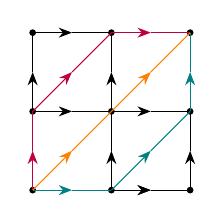
\begin{tikzpicture}
%%   vertices
   \draw[fill=black] (0,0) circle (   1pt);
   \draw[fill=black] (1,0) circle (1pt);
   \draw[fill=black] (1,1) circle (1pt);
   \draw[fill=black] (0,1) circle (1pt);
   \draw[fill=black] (0,2) circle (   1pt);
   \draw[fill=black] (1,2) circle (   1pt);
   \draw[fill=black] (2,0) circle (1pt);
   \draw[fill=black] (2,1) circle (1pt);
   \draw[fill=black] (2,2) circle (1pt);
%%% edges
   \draw[teal,-Stealth] (0,0) -- (0.5,0);
   \draw[teal] (0.5,0) -- (1,0);
   \draw[-Stealth] (1,0) -- (1.5,0);
   \draw (1.5,0) -- (2,0);
   \draw[-Stealth] (0,1) -- (0.5,1);
   \draw (0.5,1) -- (1,1);
   \draw[-Stealth] (1,1) -- (1.5,1);
   \draw (1.5,1) -- (2,1);
   \draw[-Stealth] (0,2) -- (0.5,2);
   \draw (0.5,2) -- (1,2);
   \draw[purple,-Stealth] (1,2) -- (1.5,2);
   \draw[purple] (1.5,2) -- (2,2);
   \draw[-Stealth] (1,0) -- (1.5,0);
   \draw (1.5,0) -- (2,0);
\draw[purple,-Stealth] (0,0) -- (0,0.5); \draw[purple] (0,0.5) -- (0,1);
\draw[-Stealth] (0,1) -- (0,1.5); \draw (0,1.5) -- (0,2);
\draw[-Stealth] (1,0) -- (1,0.5); \draw (1,0.5) -- (1,1);
\draw[-Stealth] (1,1) -- (1,1.5); \draw (1,1.5) -- (1,2);
\draw[-Stealth] (2,0) -- (2,0.5); \draw (2,0.5) -- (2,1);
\draw[teal,-Stealth] (2,1) -- (2,1.5); \draw[teal] (2,1.5) -- (2,2);

%%% diagonal edges
   \draw[orange,-Stealth] (0,0) -- (0.5,0.5);
   \draw[orange] (0.5,0.5) -- (1,1);
   \draw[teal,-Stealth] (1,0) -- (1.5,0.5);
   \draw[teal] (1.5,0.5) -- (2,1);
   \draw[purple,-Stealth] (0,1) -- (0.5,1.5);
   \draw[purple] (0.5,1.5) -- (1,2);
   \draw[orange,-Stealth] (1,1) -- (1.5,1.5);
   \draw[orange] (1.5,1.5) -- (2,2);

 \end{tikzpicture}
\end{figure}


The given quasi-triangulation of the torus of course lifts to a triangulation
of the universal covering $\RR^2$. The picture is obtained from
\cref{fig:torus} by periodically repeating in all directions.

The shortest combinatorial closed geodesics here have length $6$, one example
is given by concatenating the red and the green geodesics in
\cref{fig:torus}. Here, the reversing number is $2$, hence the reversing index
again is $1$. 
\end{example}

\subsection{Concluding remarks}

The fundamental identity of our work is \cref{eq:transfer_eq} which relates
the combinatorial Laplacian to the transfer operator of a random walk. In our
case, this is a signed random walk on the $n-1$-skeleton of a manifold.

As mentioned earlier, a similar approach has been used on the $0$-skeleton
(and dually also $1$-skeleton) of a regular graph (which could arise as the
$1$-skeleton of a CW-complex). There, it gives rise to an
honest (non-signed) random walk on the graph.

The key point of our approach is the packaging of the combinatorial dynamical
information in a zeta function. This encodes the spectral information in a
different way from the approach of Varopoulos
\cite{Varopoulos}. Varopoulos' result is more direct, but he uses significantly
the positivity of the random walk, which is not available in our context.

In the case of graphs and more specifically trees with a cocompact action
of a group $\pi$, there are also approaches to define and study zeta functions
and relate them to the combinatorial Laplacian. A specific example here is the
Ihara zeta function as introduced and studied by Bass in \cite{Bass92}. On a
formal level, many fundamental properties are similar to ours, compare
e.g.~\cite[Theorem 3.9]{Bass92}. On the other hand, there are also many
fundamental differences: Bass uses non-commutative determinants in the style
of Hattori--Stallings. They are finer, but much more intricate than our
Fuglede--Kadison invariant, whereas the latter can be defined and manipulated
in more general situations. Bass deals with proper actions which are not
necessarily free (free actions on trees occur only by free groups).

This leaves an interesting question in our context: can one prove suitable
generalizations of Theorem \ref{theo:mainL2} when we have a simplicial action
on a non-compact manifold $\wh M$ which is proper and cocompact, but not free
(i.e.~with finite stabilizers of simplices)? A suitable theory of
$L^2$-invariants in this context exists, see \cite[Section 6]{Lueck}.

Another question which we leave open is inspired by the work of Varopoulos
\cite{Varopoulos} and H\"opfner \cite{Hoepfner} which both get
informations about the Novikov-Shubin invariant of the manifold from the
(signed) random walk. It seems plausible the Novikov-Shubin invariant of
$\Delta_1^{(2)}$ is encoded in the behavior of the
``secondary function'' $f(z)$ of \cref{theo:mainL2} which describes the deviation
from the power function $z^{b_1^{(2)}(M,\pi)}$ of the $L^2$-zeta function near
$\frac{1}{n+2}$.


\bibliographystyle{plain} % D'autres styles sont disponibles. Notez que les distributions LaTeX n'incluent g?ï¿œn?ï¿œralement pas de styles de bibliographies francis?ï¿œs ; vous aurez donc des bibliographies en anglais.
\bibliography{biblio} % Remplacer "biblio" par le nom de votre fichier de r?ï¿œf?ï¿œrences bibliographiques.

% \begin{thebibliography}{9}
% \bibitem[Fried]{Fried}
% \textsc{Fried, D.}, \emph{Fuchsian groups and Reidemeister torsion}, in "The Selberg trace formula and related topics" (Brunswick, Maine, 1984), Contemp. Math. 53, 141-163, Amer. Math. Soc., Providence, RI, 1986.
% \bibitem[DZ]{DZ}
% \textsc{Dyatlov, S. and Zworski, M.}, \emph{Ruelle zeta function at zero for surfaces}, 	Inventiones Mathematicae 210 (2017), 211-229
 
%\end{thebibliography}

\end{document}


%%% Local Variables:
%%% mode: LaTeX
%%% TeX-master: t
%%% End:
